%% EcoPE-GAT (as-of) article, Elsevier cas-sc (single column) class, written 2026-11-21.
%% Structure, section titles and formatting follow the original manuscript
%% (paper_archive/main_before_rebuild_2026-11-16.tex).
%% Sources of the numbers: data counts from results/numbers.tex (src/07_tables.py);
%% hold-out results from reports/holdout/{scores,tests}.csv, verdicts.json and pre_prediction.json
%% (single run, tag `holdout-results`); development results from reports/dev_results/ and reports/pests/;
%% pre-registrations reports/preregistration_D13..D16.md (tags prereg-D13, prereg-D14,
%% prereg-D15-content, prereg-D16, frozen-D16). Text marked \pending{...} (red) is still to be done.
\PassOptionsToPackage{hyperfootnotes=false}{hyperref}
\documentclass[a4paper,fleqn]{cas-sc}

\usepackage[numbers,square,sort&compress]{natbib}

% No ORCID information supplied for the authors; suppress the (otherwise empty) ORCID footnote.
\RenewDocumentCommand \printorcid { } { }
\usepackage{amsmath,amssymb}
\usepackage{booktabs}
\usepackage{enumitem}
\usepackage{graphicx}
\usepackage{subcaption}
\usepackage{float}
\usepackage{placeins}
\usepackage{xcolor}
\usepackage{adjustbox}
\usepackage{algorithm}
\usepackage{algpseudocode}
\usepackage{tikz}
\usetikzlibrary{arrows.meta,positioning,patterns}

% AUTO-GENERATED by src/07_tables.py -- do not edit by hand.

\newcommand{\nPlotsTotal}{95{,}104}  % sPlotOpen plots
\newcommand{\nPlotsNoDate}{15{,}019}
\newcommand{\surveyYearMin}{1888}
\newcommand{\surveyYearMax}{2015}
\newcommand{\pctPlotsPreNineteen}{44}  % dated plots surveyed before 1999 (%)
\newcommand{\nEligible}{44{,}772}
\newcommand{\nEligibleCoords}{41{,}132}
\newcommand{\nEligibleDatasets}{93}
\newcommand{\gbifRecordsRaw}{22{,}129}
\newcommand{\gbifSpecies}{27}
\newcommand{\gbifPresent}{21{,}674}
\newcommand{\gbifUncOK}{21{,}468}
\newcommand{\gbifNoMS}{9{,}926}
\newcommand{\gbifFinal}{8{,}276}  % main variant after dedup
\newcommand{\gbifFinalAllBasis}{11{,}475}
\newcommand{\gbifFinalUncDrop}{5{,}538}
\newcommand{\pctUncMissing}{71}
\newcommand{\pctMaterialSample}{54}
\newcommand{\nMaterialSample}{12{,}001}
\newcommand{\prevNfive}{5.0}  % % positive, main, N=5
\newcommand{\nPosNfive}{2{,}231}
\newcommand{\prevAllBasisNfive}{6.7}
\newcommand{\prevNseven}{6.7}  % % positive, main, N=7
\newcommand{\nPosNseven}{3{,}007}
\newcommand{\prevAllBasisNseven}{9.7}
\newcommand{\prevNonezero}{8.5}  % % positive, main, N=10
\newcommand{\nPosNonezero}{3{,}804}
\newcommand{\prevAllBasisNonezero}{12.9}
\newcommand{\pctPrior}{5.7}
\newcommand{\prevGivenPriorNfive}{43}
\newcommand{\prevGivenNoPriorNfive}{2.7}
\newcommand{\effortOutROCNfive}{0.88}  % effort outside label window
\newcommand{\effortOutPRNfive}{0.50}
\newcommand{\priorCountPRNfive}{0.31}  % prior count as score
\newcommand{\priorCountROCNfive}{0.73}
\newcommand{\prevGivenPriorNseven}{51}
\newcommand{\prevGivenNoPriorNseven}{4.0}
\newcommand{\effortOutROCNseven}{0.86}  % effort outside label window
\newcommand{\effortOutPRNseven}{0.56}
\newcommand{\priorCountPRNseven}{0.32}  % prior count as score
\newcommand{\priorCountROCNseven}{0.70}
\newcommand{\prevGivenPriorNonezero}{57}
\newcommand{\prevGivenNoPriorNonezero}{5.5}
\newcommand{\effortOutROCNonezero}{0.81}  % effort outside label window
\newcommand{\effortOutPRNonezero}{0.51}
\newcommand{\priorCountPRNonezero}{0.32}  % prior count as score
\newcommand{\priorCountROCNonezero}{0.68}
\newcommand{\prevContNonezeroEurope}{26.4}
\newcommand{\prevContNonezeroNorthAmerica}{1.4}
\newcommand{\prevContNonezeroOceania}{13.9}
\newcommand{\nBlocks}{270}
\newcommand{\blockKm}{500}
\newcommand{\foldSizeMin}{8{,}933}
\newcommand{\foldSizeMax}{8{,}997}
\newcommand{\nFolds}{5}
\newcommand{\nSeeds}{5}
\newcommand{\nTrials}{30}
\newcommand{\tuningHorizon}{10}
\newcommand{\bufferKm}{50}
\newcommand{\kNeighbours}{10}

\newcommand{\pending}[1]{\textcolor{red}{[PENDING: #1]}}

% Model names (code names in Table~\ref{tab:models})
\newcommand{\Masof}{\mbox{EcoPE-GAT\textsubscript{as-of}}}
\newcommand{\Masofplus}{\mbox{EcoPE-GAT\textsubscript{as-of+}}}
\newcommand{\Mcausal}{\mbox{EcoPE-GAT\textsubscript{causal}}}
\newcommand{\Mleaky}{\mbox{EcoPE-GAT\textsubscript{leaky}}}
\newcommand{\Mnoctx}{\mbox{GAT\textsubscript{no-ctx}}}
\newcommand{\Lg}{\mbox{LGBM}}
\newcommand{\Lnbr}{\mbox{LGBM\textsubscript{nbr}}}
\newcommand{\Lleaky}{\mbox{LGBM\textsubscript{nbr,leaky}}}
\newcommand{\Lasof}{\mbox{LGBM\textsubscript{nbr,as-of}}}

\newtheorem{definition}{Definition}
\newtheorem{proposition}{Proposition}
\newproof{pf}{Proof}

\begin{document}
\let\WriteBookmarks\relax
\def\floatpagepagefraction{1}
\def\textpagefraction{.001}

% Short title
\shorttitle{EcoPE-GAT with as-of message passing}

% Short author
\shortauthors{Laib and Laiche}

% Main title of the paper
\title[mode=title]{As-of message passing: a leakage-free graph attention network for forecasting plant pathogen and crop pest emergence from time-stamped occurrence records}

% First author
\author[1]{Mohamed Djounaid Laib}
\ead{Mohamed.djounaid.laib_d@usthb.edu.dz}
\credit{Conceptualization, Methodology, Software, Formal analysis, Writing -- original draft}

% Second author
\author[1,2]{Nacéra Laiche}
\cormark[1]
\ead{nlaiche@usthb.dz}
\credit{Supervision, Methodology, Writing -- review \& editing}

\affiliation[1]{organization={LRIA, University of Sciences and Technology Houari Boumediene (USTHB)},
            city={Algiers},
            country={Algeria}}

\affiliation[2]{organization={Faculty of Computer Science, Artificial Intelligence and Data Sciences Department, University of Sciences and Technology Houari Boumediene (USTHB)},
            city={Algiers},
            country={Algeria}}

\cortext[1]{Corresponding author}

% Here goes the abstract
\begin{abstract}
Graph neural networks pass information between neighbouring observations. In species distribution models built from time-stamped occurrence records, a neighbour surveyed later can transmit records that fall inside the receiving site's prediction window, even under spatially blocked validation. The usual remedy, deleting edges from later neighbours, removes information together with the leak. We propose as-of message passing, which carries the point-in-time principle of temporal graph learning over to static spatial graphs: every neighbour's time-stamped features are recomputed at the receiver's date, so that all edges are kept and, as we prove, no message contains a record from the prediction window. We build on it EcoPE-GAT, a new graph attention network in which every site and every message carry an ecological positional encoding of their environmental context, and forecast new plant-pathogen records near \nEligible{} sPlotOpen vegetation plots and new records of two invasive crop pests in three regions from GBIF data. On sealed, pre-registered hold-outs, the as-of model outperformed edge deletion in two of three pest cases, was positive but inconclusive on pathogens, matched a gradient-boosting model with time-safe neighbourhood features, and outperformed persistence where the organism had not yet been recorded.
\end{abstract}

\begin{highlights}
\item Later-surveyed neighbours leak future records into graph distribution models
\item As-of message passing recomputes neighbour features at the receiver's date
\item It keeps every edge and provably passes no record from the prediction window
\item Pre-registered hold-outs: as-of beats edge deletion in 2 of 3 crop-pest cases
\item The as-of GAT matches LightGBM and beats persistence before first local records
\end{highlights}

% Keywords
\begin{keywords}
Graph Neural Network \sep Temporal Leakage \sep Message Passing \sep Plant Pathogen Emergence \sep Invasive Crop Pests \sep Ecological Positional Encoding \sep GBIF \sep sPlotOpen \sep Pre-registration
\end{keywords}

{\hfuzz=118pt\maketitle}

% =========================================================
\section{Introduction}

Plant pathogens and crop pests represent some of the most pervasive and poorly predicted threats to terrestrial ecosystems and global food security \citep{bebber2014,fisher2012}. Open data now describe both the places that are surveyed and the organisms that are reported there: vegetation-plot databases such as sPlotOpen characterise tens of thousands of plant communities \citep{sabatini2021}, and the Global Biodiversity Information Facility (GBIF) aggregates millions of dated and georeferenced occurrence records. Anticipating where a pathogen or a pest will be reported next, from what was known at a given date, is the forecasting question these data make possible.

Existing approaches exhibit two fundamental limitations for this question. First, species distribution models (SDMs) relate occurrences to environmental covariates measured at each site \citep{elith2009}, and the quantity they estimate depends on the data type and on the sampling process \citep{guillera2015}; they do not use the dated history of neighbouring sites, although the spread of an organism is a process in which this history is informative. Graph neural networks (GNNs) pass information between related sites and have recently been applied to species distribution modelling \citep{wu2025,harrell2025}. Second, occurrence-based models are confounded by surveillance effort \citep{beck2014,phillips2009}, and evaluation designs that ignore spatial structure overstate generalisation \citep{roberts2017,ploton2020}. We show that combining the two, a graph over sites surveyed at different dates, creates a third problem that spatial validation does not detect: when a node's features count the records known before its own survey date, a neighbour surveyed later passes to the receiving site records from the very window the model is asked to predict. This is temporal leakage in the sense of Kaufman et al.~\citep{kaufman2012}, but it enters through the model's input rather than through the data split.

The natural remedy, following the requirement that features use only information available at prediction time \citep{kaufman2012}, is to delete every edge from a neighbour surveyed after the receiver. It closes the leak but also discards information that was legitimately available at the receiver's date: in our pathogen graph it removes 15.2\% of the edges and isolates 232 nodes, and the corrected graph model falls behind a tabular model. We introduce instead \textbf{as-of message passing}, a message-passing rule in which the time-stamped features of every neighbour are recomputed \emph{as of the receiver's date}. Every edge is kept, every node keeps its neighbours, and no message contains a record from the receiver's future. The underlying principle, that a representation at time $t$ may only use information from before $t$, is standard in temporal graph learning \citep{xu2020tgat,rossi2020} and in point-in-time (``as-of'') feature joins; our contribution is its formulation for message passing on static proximity graphs of irregularly dated sites, where it has not been applied, together with a formal guarantee and a pre-registered evaluation. On this rule we build a new model, EcoPE-GAT (Ecological Positional Encoding Graph Attention Network). Its nodes are dated sites; the receiving site and every message carry a learned encoding of the ecological context of their site (climate, location, biome), because a geographic graph says which sites are close but not which environment they share; and attention weighs messages computed as of the receiver's date. We write \Masof{} for the proposed model when it must be distinguished from two ablations that share its encoder and readout but use standard graph attention layers on the stored features: \Mleaky{} on all edges and \Mcausal{} after edge deletion.

We evaluate \Masof{} on two forecasting problems built from GBIF: new plant-pathogen records near \nEligible{} sPlotOpen vegetation plots, and new records of two invasive crop pests, \textit{Halyomorpha halys} in Europe and North America and \textit{Popillia japonica} in North America \citep{leskey2018,althoff2022}. All hypotheses were pre-registered and tested once on sealed hold-out data \citep{nosek2018}, and all outcomes are reported, including those that do not support our expectations.

Our main contributions are:
\begin{enumerate}[leftmargin=1.4em]
  \item EcoPE-GAT, a graph attention network for forecasting the emergence of an organism at dated sites, in which the receiver and every message carry an ecological positional encoding (EcoPE) of their site and attention operates on messages computed as of the receiver's date.
  \item As-of message passing, a formulation of the point-in-time principle for message passing on static proximity graphs whose nodes carry cumulative time-stamped features, with a proof that no message contains information from the receiver's prediction window and a complexity analysis; the same rule also yields time-safe neighbourhood features for tabular models.
  \item A formal characterisation of temporal leakage through neighbours in graph SDMs, a proof that the edge-deletion rule holds over several message-passing layers, and a three-level diagnostic that other authors can apply.
  \item Two reproducible forecasting benchmarks: sPlotOpen plots linked to a single citable GBIF download of \gbifSpecies{} plant-pathogen species with an independent sampling-effort layer, and three crop-pest cases built from GBIF records.
  \item A pre-registered confirmatory evaluation on sealed hold-outs. The as-of model outperformed edge deletion in two of three pest cases, matched the strongest tabular reference, and outperformed a persistence baseline at sites without prior records; the leakage itself inflated hold-out performance only for pathogens in one of two settings.
\end{enumerate}

The remainder of this paper is organised as follows. Section~\ref{sec:relwork} reviews related work on functional-trait-based pathogen prediction, graph neural networks for ecological modelling, positional encoding in GNNs, and spatial evaluation bias and leakage, before summarising the resulting research gap. Section~\ref{sec:approach} presents our proposed approach: the motivation, the construction of the datasets, the EcoPE-GAT architecture with its as-of message passing and their formal properties, and how predictions are produced. Section~\ref{sec:expsetup} describes the pre-registered evaluation protocol, baselines, implementation details and results. Section~\ref{sec:discussion} discusses the implications, ecological interpretation and limitations of our findings, and Section~\ref{sec:conclusion} concludes the paper.

% =========================================================
\section{Related Work}
\label{sec:relwork}

Work related to ours can be organised into four broad families: (1)~approaches to plant disease and pathogen risk prediction from functional traits and occurrence records, which define the forecasting task; (2)~graph neural networks applied to ecological and species distribution modelling, which motivate our architectural choice of GAT; (3)~positional encoding strategies for graph neural networks, which contextualise the EcoPE encoder; and (4)~work on spatial generalisation, evaluation bias and leakage, including temporal leakage in graph learning, which motivates as-of message passing. We review each family in turn before summarising the specific gap that our work addresses.

\subsection{Functional-trait based pathogen prediction}

Plant pathogens are increasingly recognised as a direct threat to global food security and ecosystem stability \citep{bebber2014}, with fungal and fungal-like pathogens responsible for a growing share of emerging infectious disease events across plant, animal and ecosystem health \citep{fisher2012}. Plant functional traits link the response of plant communities to environmental factors with their effects on ecosystem functioning \citep{lavorel2002}, and the global relationships between community-level traits and climate and soil have been quantified from vegetation plots \citep{bruelheide2018}. Host traits shape plant responses to pathogen stress at the individual level \citep{jin2021}, and host community traits modulate disease risk along environmental gradients \citep{halliday2021}. Representation-learning alternatives have also been proposed, such as species embeddings learned from co-occurrence on sPlotOpen \citep{siefert2024}. Correlative SDMs remain the standard tool for predicting distributions across space and time \citep{elith2009}; what they estimate depends on the data type and on imperfect detection and sampling bias \citep{guillera2015}, and their transferability to novel conditions is an open challenge \citep{yates2018}. For invasive crop pests, occurrence records document a spread front that moves over years, as for the brown marmorated stink bug \textit{H. halys} in Europe and North America \citep{leskey2018} and the Japanese beetle \textit{P. japonica} in North America \citep{althoff2022}.

Existing approaches model sites independently and rely on covariates measured at the site itself; they do not exploit the dated history of neighbouring sites, which is precisely the information that describes a spreading organism.

\subsection{Graph Neural Networks for Ecological Modelling}

Gradient-boosted trees and random forests remain strong baselines for tabular ecological data \citep{valavi2022} and often outperform deep learning on tabular benchmarks \citep{grinsztajn2022}. Graph neural networks add a mechanism for exploiting relations between observations. Graph Convolutional Networks (GCN) aggregate neighbour information using fixed, normalised weights \citep{kipf2017}; GraphSAGE learns aggregation functions that apply to previously unseen nodes \citep{hamilton2017}; and Graph Attention Networks (GAT) learn per-edge attention coefficients, offering an interpretable weighting of each neighbour's contribution \citep{velickovic2018}. This family of models has recently been applied directly to species distribution modelling: Wu et al.~\citep{wu2025} propose GNN-SDM, which aggregates environmental layers into landscape patches and infers habitat suitability from IUCN range polygons, and Harrell et al.~\citep{harrell2025} introduce a heterogeneous GNN with species and locations as two node sets, which is comparable to or better than single-species SDMs and a feed-forward baseline on a standard benchmark. Spatio-temporal graph models have also been used to forecast the spread of a forest pest, \textit{Dendroctonus valens}, across Chinese counties \citep{zhou2026}, and to learn joint species distributions from dynamic habitat context and community structure \citep{kong2026}.

These ecological GNNs either treat node features as static or operate on units observed at common time steps; none of them addresses graphs whose nodes are surveyed at different, irregular dates, where the features of a neighbour may postdate the node that receives them.

\subsection{Positional Encoding in Graph Neural Networks}

GNN positional encodings provide each node with information that message passing alone cannot recover. Laplacian eigenvector encodings \citep{dwivedi2020} and distance-based structural encodings \citep{li2020} describe a node's position in the graph topology. Closer to our setting, Klemmer et al.~\citep{klemmer2023pegnn} propose PE-GNN, which learns an embedding of raw geographic coordinates for spatial regression on proximity graphs, and Zhao and Efremova~\citep{zhao2023} apply this paradigm to soil organic carbon estimation from climate features.

These encoders embed coordinates or graph structure; an encoding of the ecological context of each node (climate, coordinates and biome), applied to both the receiver and its neighbours before message passing, is the role of the EcoPE encoder in our model. Whether such an encoder adds anything over concatenating the same variables is an empirical question, which we treat as a tuned choice.

\subsection{Spatial Generalisation and Evaluation Bias}

Robust evaluation is a persistent methodological challenge in spatial ecological modelling. Random cross-validation overestimates predictive performance when observations are spatially autocorrelated, and spatially blocked or geographically structured hold-outs give more honest estimates \citep{roberts2017,hijmans2012,valavi2019,ploton2020}; the same holds for spatio-temporal models \citep{meyer2018}, although spatial cross-validation can also be pessimistic for map accuracy \citep{wadoux2021}. In spatio-temporal GNNs for epidemic forecasting, all locations remain in the graph during training and prediction \citep[e.g.][]{croft2023}. More generally, leakage, the introduction of information about the target that should not legitimately be available, is formalised by Kaufman et al.~\citep{kaufman2012}; Kapoor and Narayanan~\citep{kapoor2023} found leakage in 294 papers across 17 fields and proposed a taxonomy of eight types. For graph models, a recent re-evaluation of fraud detection on a Bitcoin transaction graph attributed much of the reported advantage of GNNs to training-time exposure to the test-period graph \citep{maganti2026}. In temporal graph learning, the principle that a representation at time $t$ uses only earlier information is built into the models: JODIE updates embeddings at each interaction \citep{kumar2019}, TGAT aggregates temporal neighbourhood features with a functional time encoding \citep{xu2020tgat}, and Temporal Graph Networks operate on sequences of timed events \citep{rossi2020}; benchmark studies further show that evaluation choices strongly affect the ranking of dynamic-graph models \citep{poursafaei2022,huang2023}. In data engineering, point-in-time (``as-of'') joins serve the same purpose for tabular features.

This literature addresses leakage through the data split, through the test-period graph, or through time-stamped events in dynamic graphs. Graph SDMs are usually built as static proximity graphs over observations made at different dates, with cumulative dated features stored once per node; we found no study that tests for, or constrains, the timing of the information that neighbours pass to each other in this setting.

\subsection{Summary of Research Gap}

As far as we know, no existing work simultaneously: (1)~forecasts the emergence of plant pathogens or crop pests as node classification on a graph of dated sites, (2)~characterises the temporal leakage that time-stamped node features create through message passing, even under spatially blocked validation, (3)~transfers the point-in-time principle of temporal graph learning to message passing on such static graphs, removing the leakage without deleting edges and with a formal guarantee, and (4)~tests the resulting model against strong tabular references on sealed, pre-registered hold-outs. Our objective is therefore to develop a graph model for emergence forecasting whose messages are, by construction, restricted to information available at each site's prediction date. To achieve this objective, we propose EcoPE-GAT, a graph attention network with an ecological positional encoding whose message passing is as-of (\Masof).

% =========================================================
\section{Proposed Approach}
\label{sec:approach}

\subsection{Motivation}
\label{sec:motivation}

Before describing the architecture in detail, we lay out the three observations that motivate its design, and briefly recall the graph neural network background that informs our choice of backbone.

\textbf{Observation 1: the dated history of neighbouring sites is predictive.} In our development data, the strongest predictors of a new record within $N$ years are the records already known near the site and near its neighbours before the survey date, together with sampling effort and location (Section~\ref{sec:dataset}). A LightGBM model that adds time-safe aggregates of its geographic neighbours (\Lnbr) is the best admissible model on the pathogen development data.

\textbf{Observation 2: a neighbour surveyed later leaks the receiver's future.} A node's prior-presence features count the records known before \emph{its own} survey year. In a graph over plots surveyed in different years, a neighbour $j$ surveyed after plot $i$ therefore carries records from $i$'s prediction window (Figure~\ref{fig:leak}). In the development pathogen graph, 15.2\% of the directed edges come from a later-surveyed neighbour; 30.2\% of positive plots receive such a message against 0.5\% of negative plots, and this indicator alone ranks plots with a PR-AUC of 0.27 at a prevalence of 0.05. The leak passes through the model input, so a spatially blocked split does not prevent it.

\textbf{Observation 3: deleting later neighbours removes information as well as the leak.} Restricting messages to neighbours surveyed no later than the receiver removes 15.2\% of the edges, reduces the median in-degree from 12 to 10 and leaves 232 nodes (0.6\%) without any neighbour. On the development data, the corrected graph model (\Mcausal) has a spatial cross-validation PR-AUC of 0.364, against 0.478 for the same model on the original graph and 0.456 for \Lnbr.

These observations motivate a message-passing rule that keeps every neighbour but evaluates what each neighbour knows at the receiver's date.

\begin{figure}[pos=t]
  \centering
  \resizebox{\linewidth}{!}{%
  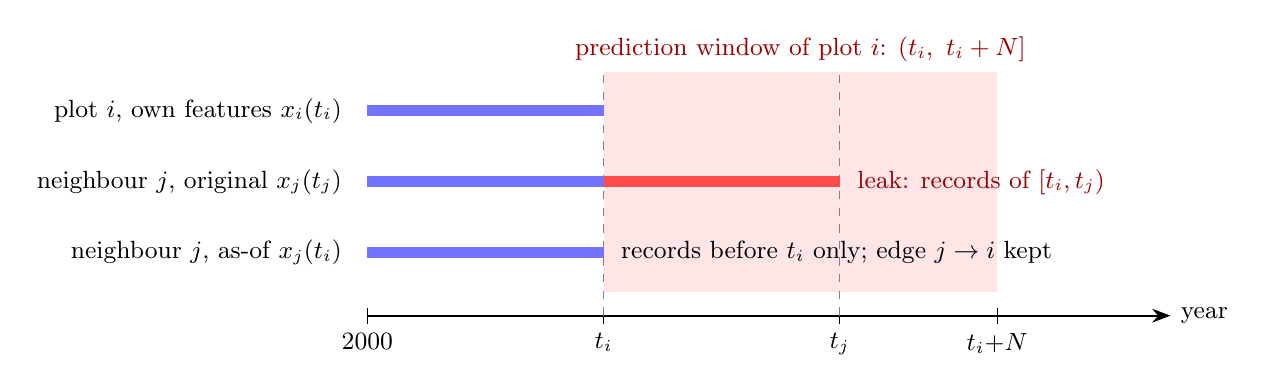
\begin{tikzpicture}[font=\small]
    % label window of plot i
    \fill[red!10] (3,-0.3) rectangle (8,2.5);
    \node[red!60!black,anchor=south] at (5.5,2.5) {prediction window of plot $i$: $(t_i,\ t_i+N]$};
    % time axis
    \draw[-{Stealth},thick] (0,-0.6) -- (10.2,-0.6) node[right] {year};
    \foreach \x/\lab in {0/2000,3/$t_i$,6/$t_j$,8/$t_i{+}N$} {
      \draw (\x,-0.5) -- (\x,-0.7) node[below] {\lab};
    }
    \draw[dashed,gray] (3,-0.6) -- (3,2.5);
    \draw[dashed,gray] (6,-0.6) -- (6,2.5);
    % plot i
    \node[anchor=east] at (-0.2,2.0) {plot $i$, own features $x_i(t_i)$};
    \draw[line width=4pt,blue!55] (0,2.0) -- (3,2.0);
    % neighbour j, original features
    \node[anchor=east] at (-0.2,1.1) {neighbour $j$, original $x_j(t_j)$};
    \draw[line width=4pt,blue!55] (0,1.1) -- (3,1.1);
    \draw[line width=4pt,red!70] (3,1.1) -- (6,1.1);
    \node[anchor=west,red!60!black] at (6.1,1.1) {leak: records of $[t_i, t_j)$};
    % neighbour j, as-of features
    \node[anchor=east] at (-0.2,0.2) {neighbour $j$, as-of $x_j(t_i)$};
    \draw[line width=4pt,blue!55] (0,0.2) -- (3,0.2);
    \node[anchor=west] at (3.1,0.2) {records before $t_i$ only; edge $j \to i$ kept};
  \end{tikzpicture}}
  \caption{Temporal leakage through a neighbour and its as-of correction. Bars show the years of records counted in a time-stamped feature. Plot $i$, surveyed in year $t_i$, is to be labelled from records in $(t_i, t_i+N]$. Its neighbour $j$, surveyed in year $t_j > t_i$, counts records before $t_j$ (red: inside $i$'s window). Edge deletion removes the edge $j \to i$; as-of message passing keeps it and recomputes $j$'s features at $t_i$.}
  \label{fig:leak}
\end{figure}

\subsubsection{GNNs and Graph Attention Networks: Background}
\label{sec:gat-background}

Among graph neural network architectures, Graph Convolutional Networks aggregate neighbour information using fixed, normalised weights, and GraphSAGE learns flexible aggregation functions without per-edge weights. Graph Attention Networks extend this idea by learning, for each edge $(j,i)$, an attention coefficient $\alpha_{ji}$ that weights the contribution of neighbour $j$ to node $i$'s representation \citep{velickovic2018}.

This property is particularly well suited to our setting: not all neighbours of a site are equally informative, and a neighbour with a recent record of the organism nearby should contribute more to a site's risk than a neighbour without any. We therefore adopt attention as the aggregation mechanism of the proposed model, and describe in Section~\ref{sec:architecture} how messages are built so that this attention operates only on information available at the receiver's date.

\subsection{Methodology}
\label{sec:overview}

Our pipeline comprises three steps: (i)~constructing the forecasting datasets from sPlotOpen and GBIF records, with dated node features and sealed hold-outs (Section~\ref{sec:dataset}); (ii)~building the EcoPE-GAT architecture, which combines a geographic graph, the EcoPE encoder and as-of message passing (Section~\ref{sec:architecture}); and (iii)~producing site-level emergence predictions (Section~\ref{sec:predictions}). EcoPE-GAT, and its as-of message passing in particular, is the central modelling component of this pipeline and the primary contribution of this work; the dataset construction and prediction steps are necessary supporting stages.

\subsubsection{Dataset Construction}
\label{sec:dataset}

\begin{itemize}[leftmargin=1.4em]

\item \textbf{Vegetation Plot Database.} The nodes of the pathogen task are vegetation plots from sPlotOpen \citep{sabatini2021,splotdata}, which contains \nPlotsTotal{} plots surveyed between \surveyYearMin{} and \surveyYearMax. Survey year was parsed from the recording date; \nPlotsNoDate{} plots without a date were excluded. For each plot we retained latitude and longitude, the two soil--climate principal components provided with the data (SoilClim PC1 and PC2), biome (ten zones) and survey year $t_i$.

\item \textbf{Pathogen Occurrence Records and Spatial Joining.} Pathogen occurrences come from a single GBIF download of \gbifRecordsRaw{} records of \gbifSpecies{} plant-pathogen species recorded between 2000 and 2025 \citep{gbifdownload}. We kept records with occurrenceStatus PRESENT, valid non-zero coordinates and a coordinate uncertainty of at most 10~km (\pctUncMissing\% of the records have no uncertainty value and were kept), removed records with basisOfRecord MATERIAL\_SAMPLE, which are mostly environmental-DNA detections rather than reports on plants (\pctMaterialSample\% of the download), and removed duplicates (same species, coordinates rounded to 0.01\textdegree, same year), leaving \gbifFinal{} records. Plots and records were joined by great-circle distance within a buffer of \bufferKm~km.

\item \textbf{Emergence Labels and Class Imbalance.} Given a plot $i$ surveyed in year $t_i$, its label under horizon $N$ is
\begin{equation}
y_i^{(N)} = \mathbb{1}\Big[\exists\ r \in \mathcal{B}_i : t_i < \tau_r \leq t_i + N \Big],
\label{eq:label}
\end{equation}
where $y_i^{(N)} \in \{0,1\}$ is the emergence label of plot $i$ for horizon $N$; $\mathcal{B}_i$ is the set of filtered records within \bufferKm~km of the plot; $\tau_r$ is the year of record $r$; and $N \in \{5, 7, 10\}$ years. Because GBIF coverage starts in 2000, a plot is eligible only if its whole window lies within 2000--2025 ($t_i \geq 1999$ and $t_i + N \leq 2025$), which leaves the same \nEligible{} plots for all horizons. The positive class comprises \prevNfive\%, \prevNseven\% and \prevNonezero\% of eligible plots at $N = 5$, 7 and 10. This imbalance is addressed by weighting the positive class at $w^+ = n^-/n^+$ in the loss of the neural models and by reporting PR-AUC as the primary metric \citep{saito2015}.

\item \textbf{Time-stamped Node Features and Independent Effort.} For a plot $j$ and any date $s$, we define the time-stamped features $x_j(s)$ as computed from the records with year $< s$ only: $\log(1+n)$ of the number $n$ of target records within \bufferKm~km, the number of distinct target species among them, and an indicator $\mathbb{1}[n > 0]$. Sampling effort is measured independently of the targets, as the number of non-target fungal GBIF records in the 0.5\textdegree{} cells within \bufferKm~km of the plot in the years 2000 to $s-1$ (log-transformed), from a separate SQL download \citep{gbifeffort}. The node features of plot $j$ are $x_j = x_j(t_j)$, and records from the survey year itself are used neither as features nor as labels. Static covariates (coordinates, SoilClim PCs, biome) form the ecological context $c_j$.

\item \textbf{Evidence of a Learnable Signal.} Before introducing the graph model, we verified which variables carry predictive signal on the development data. In a default-hyperparameter pilot (spatial cross-validation, $N=5$), plant functional traits added nothing once prior presence, effort and location were known: LightGBM with traits minus LightGBM without traits $-0.013$ PR-AUC, 95\% block-bootstrap interval $[-0.088, +0.018]$, and traits predicted the continent with 72\% balanced accuracy. Traits are therefore not used in the models below. Prior presence alone ranks plots with a PR-AUC of \priorCountPRNfive{} at $N=5$; among the \pctPrior\% of plots with a prior record, \prevGivenPriorNfive\% are positive, against \prevGivenNoPriorNfive\% among plots without one. The task is thus a forecasting problem in which the dated records of the site and of its surroundings are the main source of information, which motivates a graph over geographic neighbours.

\item \textbf{Crop-pest Replication Data.} To test whether the findings replicate with independent data, regions and taxa, we built three crop-pest cases from GBIF records retrieved with the public occurrence API (coordinates present, no geospatial issue, status PRESENT): \textit{H. halys} in Europe (P1) and in North America (P2), and \textit{P. japonica} in North America (P3) \citep{leskey2018,althoff2022}. Nodes are sampling events: background records of the same insect order (Hemiptera or Coleoptera, without the target), sampled at random per country and year (seed 0) for years $t_i \in [2008, 2025-N]$, with a fixed random subsample of 30{,}000 nodes per case. The label is defined as in Equation~\eqref{eq:label} with a 50~km buffer; the primary horizon is $N = 3$ years, because invasions are fast, and $N = 5$ is secondary. Node features are the prior target count within 50~km, its indicator and the number of years with a prior record; effort is the number of background records of the node's GADM level-2 district in the years 2005 to $t_i - 1$; the context is WorldClim 2.1 bio1, bio5, bio6 and bio12 \citep{fick2017} and the coordinates. A fifth candidate, \textit{Spodoptera frugiperda} in Africa, was dropped before any analysis because only about 260 records were available in its region of emergence. \pending{register the three pest downloads as GBIF derived datasets and cite their DOIs.}

\item \textbf{Sealed Hold-out and Splits.} Plots were grouped into spatial blocks of approximately $\blockKm \times \blockKm$~km. For pathogens, a sealed hold-out of 7{,}920 plots in 92 blocks (17.7\%; random blocks stratified by continent and by tercile of block-median effort) was drawn before the development of the models reported here, and its plot identifiers were fixed by a SHA-256 checksum; the remaining 36{,}852 plots in 178 blocks form the development set, with five spatial folds. Blocks of the hold-out whose median effort equals the development threshold (no prior non-target fungal record) form its low-effort part: 3{,}629 plots in 27 blocks. For each pest case, 20\% of the blocks (stratified on block prevalence) form the sealed hold-out, built and checksummed before any model was fitted: 5{,}730 nodes in 19 blocks (P1), 7{,}393 in 33 (P2) and 5{,}599 in 20 (P3).

\end{itemize}

% =========================================================
\subsubsection{EcoPE-GAT Architecture}
\label{sec:architecture}

EcoPE-GAT has three components: an ecological positional encoder (EcoPE), which embeds the environmental context of each site; a graph attention layer, which aggregates messages from geographic neighbours; and a readout, which maps the result to the probability of a new record (Figure~\ref{fig:ecopegat}). We describe it in five steps: we formalise the task and the graph; we write the standard form of graph attention and show that, on dated sites, it creates a temporal leak, which the usual edge-deletion rule removes at a cost; we introduce as-of message passing and prove its properties; and we define the EcoPE encoder and the attention layer of EcoPE-GAT.

\begin{figure}[pos=t]
  \centering
  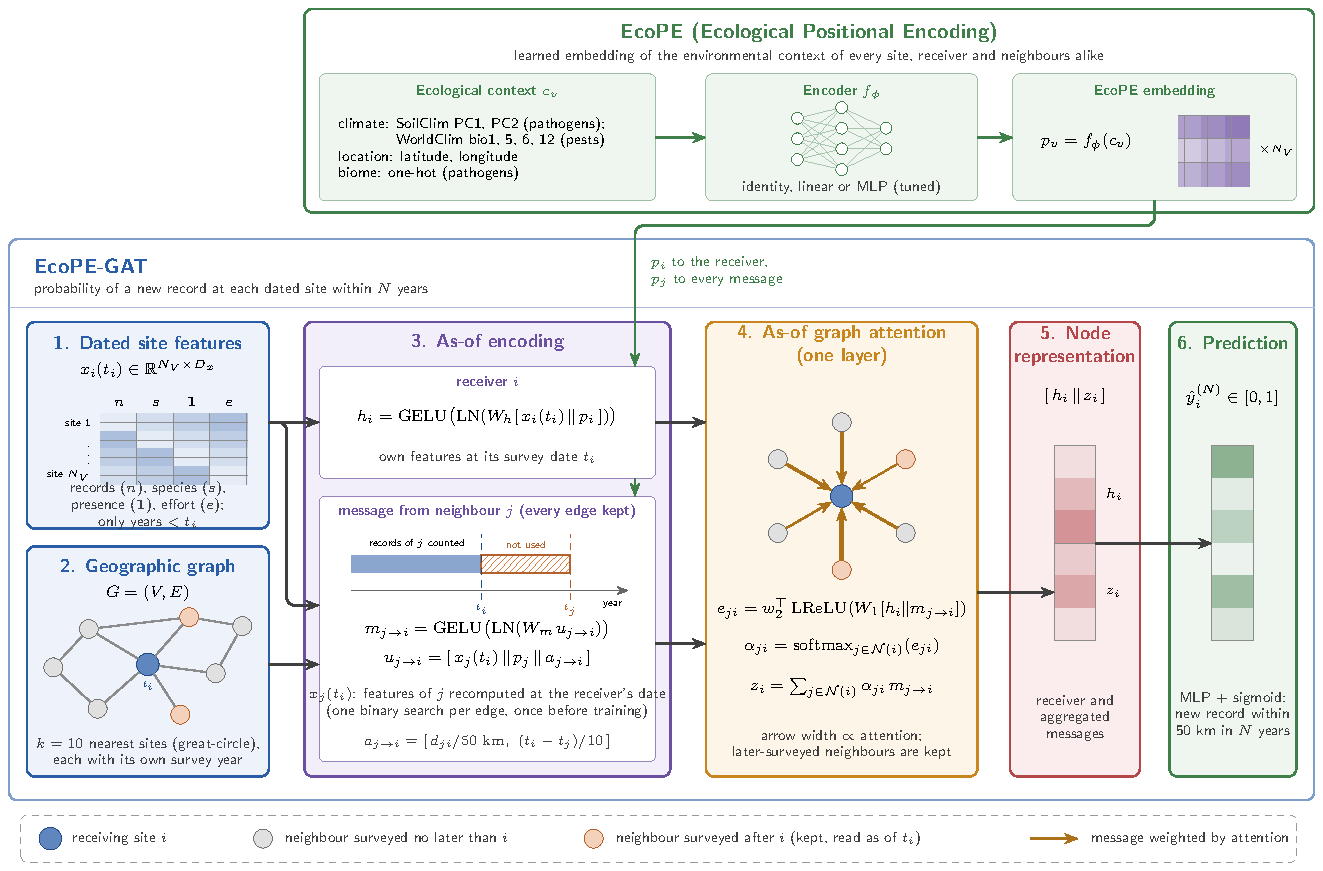
\includegraphics[width=\linewidth]{figures/ecope_gat_architecture.pdf}
  \caption{Overall architecture of EcoPE-GAT. (1)~Each site carries time-stamped features computed from records before its survey year $t_i$ and (2)~is connected to its $k$ nearest geographic neighbours, which may have been surveyed earlier or later. The EcoPE encoder (top) maps the ecological context of every site to an embedding $p_v$. (3)~The receiver embedding $h_i$ combines the receiver's features and $p_i$; for each neighbour $j$, the message $m_{j\to i}$ is built from $j$'s features recomputed at the receiver's date, $x_j(t_i)$, its embedding $p_j$ and the edge attributes, so that records of $j$ from $t_i$ onwards are not used and no edge is removed. (4)~One attention layer weighs the messages, and (5,~6)~an MLP readout on $[h_i \,\|\, z_i]$ gives the probability of a new record within $N$ years.}
  \label{fig:ecopegat}
\end{figure}

\begin{itemize}[leftmargin=1.4em]

\item \textbf{Problem Formulation and Graph Construction.} Let $G=(V,E)$ be a directed graph where each node $i \in V$ is a site with survey year $t_i$, time-stamped feature function $x_i(\cdot)$ and static context $c_i$. The task is binary node classification: predict $y_i^{(N)}$ from information available at $t_i$. Each site is connected to its $k = \kNeighbours$ nearest neighbours by great-circle distance; the graph is symmetrised, so that it contains $j \to i$ and $i \to j$, and each edge has the weight
\begin{equation}
w_{ji} = \frac{1}{1 + d_{ji}/50\ \text{km}},
\end{equation}
where $d_{ji}$ is the great-circle distance between sites $j$ and $i$. The graph is transductive: development and hold-out nodes are present, and hold-out labels are never used. Node set, coordinates, survey dates and the context $c$ are treated as carrying no information about the targets (assumption A1; Section~\ref{sec:limitations}).

\item \textbf{Standard Graph Attention.} In its standard form, graph attention would process EcoPE-GAT's inputs as follows. The node features are concatenated with the EcoPE embedding $p_i$ of the node's context, $\tilde{x}_i = [x_i \,\|\, p_i]$, and projected to width $h$ by a linear layer with layer normalisation and GELU, giving $h_i^{(0)}$. Two GAT layers then update the node representations:
\begin{align}
e_{ij}^{(l)} &= \mathrm{LeakyReLU}\big(a^\top [W h_i^{(l)} \,\|\, W h_j^{(l)} \,\|\, W_e w_{ji}]\big), \qquad
\alpha_{ij}^{(l)} = \frac{\exp(e_{ij}^{(l)})}{\sum_{k \in \mathcal{N}(i)} \exp(e_{ik}^{(l)})}, \\
h_i^{(l+1)} &= \mathrm{ELU}\Big(\big\|_{m=1}^{H} \sum_{j \in \mathcal{N}(i)} \alpha_{ij}^{(l,m)} W^{(m)} h_j^{(l)}\Big),
\end{align}
where $e_{ij}^{(l)}$ is the unnormalised attention score assigned by node $i$ to neighbour $j$ in layer $l$; $W$ is a learned projection shared across nodes, $a$ a learned attention vector and $W_e$ a projection of the edge weight $w_{ji}$; $\alpha_{ij}^{(l)}$ is the attention coefficient normalised over the neighbourhood $\mathcal{N}(i)$ (self-loops included); and $\|_{m=1}^{H}$ concatenates the outputs of $H$ heads of $h/H$ channels each. A readout MLP maps $h_i^{(2)}$ to the predicted probability. Applied to the stored dated features $x_j = x_j(t_j)$, this standard form gives the two ablations of EcoPE-GAT used as references: \Mleaky{} on the original graph and \Mcausal{} on the causal graph defined below. Because each of its two layers propagates neighbours' stored features, it is exposed to the leak described next, which motivates the as-of layer of EcoPE-GAT.

\item \textbf{Temporal Leakage through Neighbours.} In a message-passing model the representation of node $i$ depends on its neighbours' features. We call a message $j \to i$ \emph{leaking} if it is a function of a record with year $\geq t_i$, that is, of information not available at the prediction date; it carries label information when such a record falls in $(t_i, t_i+N]$.

\begin{definition}[Original and causal graphs]
With original features, the message $j \to i$ is computed from $x_j(t_j)$. The causal graph $E_c = \{(j,i) \in E : t_j \leq t_i\}$ keeps only the edges from neighbours surveyed no later than the receiver.
\end{definition}

\begin{proposition}[Leakage of the original graph and the causal rule]
\label{prop:causal}
(a) In the original graph, an edge $j \to i$ can leak only if $t_j > t_i$; it can carry a record of $i$'s prediction window only if $t_j \geq t_i + 2$. (b) In the causal graph, after $L \geq 1$ message-passing layers, every time-stamped quantity reaching node $i$ is computed from records with year $< t_i$.
\end{proposition}

\begin{pf}
(a) $x_j(t_j)$ counts records with year $< t_j$. If $t_j \leq t_i$, all of them have year $< t_i$. Otherwise the records with year in $[t_i, t_j)$ are counted, and the window $(t_i, t_i+N]$ contains one of these years only if $t_i + 1 \leq t_j - 1$. (b) After $L$ layers, $h_i$ depends on the features of the nodes $j_0$ of directed paths $j_0 \to j_1 \to \dots \to j_L = i$ in $E_c$ (self-loops included). Along such a path $t_{j_0} \leq t_{j_1} \leq \dots \leq t_i$, so every time-stamped quantity of $j_0$ uses records with year $< t_{j_0} \leq t_i$. The weaker rule ``$t_j \leq t_i + 1$'', which by (a) excludes window records over one layer, is not closed under composition: over two layers it admits paths with $t_{j_0} = t_i + 2$.
\end{pf}

The causal rule is a sufficient condition, but it deletes every edge with $t_j > t_i$, even though most of the information of such a neighbour (its records before $t_i$) was available at the receiver's date.

\item \textbf{As-of Message Passing.} The leak does not come from the neighbour itself but from the date at which its features are evaluated. As-of message passing keeps every edge and evaluates the neighbour's time-stamped features at the receiver's date:
\begin{equation}
x_{j \to i} = x_j(t_i), \qquad a_{j \to i} = \big[\,d_{ji}/50\ \text{km},\ (t_i - t_j)/10\,\big],
\label{eq:asof}
\end{equation}
where $x_{j \to i}$ is the as-of feature vector of edge $j \to i$, computed with the same definition as the node features but from records with year $< t_i$; and $a_{j \to i}$ are the edge attributes, the scaled distance and the signed difference of survey years. For $j = i$ the as-of features reproduce the node features exactly, $x_i(t_i) = x_i$, so that node and edge features share one definition. Algorithm~\ref{alg:asof} gives the complete forward pass.

\begin{proposition}[As-of message passing is leak-free and keeps every edge]
\label{prop:asof}
With one as-of attention layer (Equations~\eqref{eq:asof}--\eqref{eq:readout}), (a) every time-stamped quantity that enters the prediction $\hat{y}_i$ is computed from records with year $< t_i$, for every edge of $E$; (b) no edge is removed and no node is isolated: the in-degree of every node equals its in-degree in $G$, whereas the causal graph removes $|\{(j,i) \in E : t_j > t_i\}|$ edges.
\end{proposition}

\begin{pf}
(a) The prediction $\hat{y}_i$ is a function of $h_i$ and of the messages $m_{j \to i}$ (Equation~\eqref{eq:readout}). $h_i$ depends on $x_i = x_i(t_i)$ and $c_i$; $m_{j \to i}$ depends on $x_j(t_i)$, $c_j$ and $a_{j \to i}$; the attention coefficients depend only on $h_i$ and $m_{j \to i}$. The only time-stamped quantities are $x_i(t_i)$ and $x_j(t_i)$, which by definition count records with year $< t_i$; $c$, $d_{ji}$ and $t_i - t_j$ are covariates under assumption A1. (b) The layer aggregates over all in-edges of $G$, and $k \geq 1$ gives every node at least one in-edge.
\end{pf}

The guarantee is exact for one layer. With two layers, the message from $j$ to $i$ would contain $j$'s own aggregate of its neighbours, whose features would have to be evaluated at the date of the final receiver along each path; we therefore use a single attention layer, and the second-hop information is supplied by the as-of features themselves, which count records in a 50~km buffer around each neighbour.

\textit{Complexity.} For each node $j$ the years of its buffer records are sorted once, and the effort counts are stored as cumulative sums over years. The as-of count of an edge is then one binary search, and the as-of effort one table lookup, so that the edge features cost $O(|E| \log R_{\max} + |V|\,Y)$ time, where $R_{\max}$ is the largest number of records in a buffer and $Y$ the number of years, and $O(|E|\,d)$ memory for $d$ edge features. They are computed once, before training. The attention layer costs $O(|E|\,h)$ per forward pass for hidden width $h$, the same order as one GAT layer. The pathogen development graph has 459{,}584 directed edges; edge deletion would keep 389{,}780 of them.

\begin{algorithm}[t]
\caption{As-of message passing in \Masof{} (one forward pass; pathogen features, pests use the analogous variables of Section~\ref{sec:dataset}).}
\label{alg:asof}
\begin{algorithmic}[1]
\Require graph $E$; survey years $t$; per-node sorted record years $R_j$ and first years per species $F_j$; cumulative effort tables $P_j$; node features $x$; context $c$
\For{each edge $(j \to i) \in E$} \Comment{once, before training}
  \State $n \gets |\{r \in R_j : r < t_i\}|$ \Comment{binary search}
  \State $s \gets |\{f \in F_j : f < t_i\}|$; \quad $e \gets P_j[t_i - 2000]$
  \State $x_{j \to i} \gets [\log(1+n),\ s,\ \mathbb{1}[n>0],\ \log(1+e)]$; \quad $a_{j \to i} \gets [d_{ji}/50,\ (t_i - t_j)/10]$
\EndFor
\State $p_v \gets f_\phi(c_v)$ for all $v \in V$ \Comment{EcoPE}
\State $h_i \gets \mathrm{GELU}(\mathrm{LN}(W_h [x_i \,\|\, p_i]))$ for all $i$
\State $m_{j \to i} \gets \mathrm{GELU}(\mathrm{LN}(W_m [x_{j \to i} \,\|\, p_j \,\|\, a_{j \to i}]))$ for all $(j \to i) \in E$
\State $\alpha_{ji} \gets \mathrm{softmax}_{j \in \mathcal{N}(i)}\big(w_2^\top \mathrm{LeakyReLU}(W_1 [h_i \,\|\, m_{j \to i}])\big)$
\State $z_i \gets \sum_{j \in \mathcal{N}(i)} \alpha_{ji}\, m_{j \to i}$
\State \Return $\hat{y}_i \gets \sigma\big(\mathrm{MLP}([h_i \,\|\, z_i])\big)$ for all $i$
\end{algorithmic}
\end{algorithm}

\item \textbf{Ecological Positional Encoding (EcoPE).} The ecological context $c_v$ of every node (SoilClim PC1 and PC2, latitude, longitude and one-hot biome for pathogens; WorldClim bio1, bio5, bio6, bio12, latitude and longitude for pests) is mapped by an encoder $f_\phi$ to a positional embedding,
\begin{equation}
p_v = f_\phi(c_v),
\end{equation}
where $p_v$ is the ecological positional encoding of node $v$. In the first configuration of EcoPE-GAT explored during development, $f_\phi$ was a two-layer MLP (64 and 32 units, each with layer normalisation and GELU). Because a pre-registered development test found no advantage of this encoder over plain concatenation (Section~\ref{sec:history}), the encoder form is a tuned hyperparameter: identity (concatenation of $c_v$), linear (to 32 dimensions) or MLP. The encoder is applied to the receiver and to each neighbour before message passing, so that a message carries the ecological position of its sender.

\item \textbf{As-of Graph Attention Layer.} The receiver embedding, the messages and the attention coefficients of EcoPE-GAT are
\begin{align}
h_i &= \mathrm{GELU}\big(\mathrm{LN}(W_h [x_i \,\|\, p_i])\big), \qquad
m_{j \to i} = \mathrm{GELU}\big(\mathrm{LN}(W_m [x_{j \to i} \,\|\, p_j \,\|\, a_{j \to i}])\big), \label{eq:msg}\\
e_{ji} &= w_2^\top\, \mathrm{LeakyReLU}\big(W_1 [h_i \,\|\, m_{j \to i}]\big), \qquad
\alpha_{ji} = \frac{\exp(e_{ji})}{\sum_{l \in \mathcal{N}(i)} \exp(e_{li})}, \label{eq:att}
\end{align}
where $h_i$ is the embedding of receiver $i$; $m_{j \to i}$ is the message of edge $j \to i$; $W_h$, $W_m$, $W_1$ and $w_2$ are learned parameters (with biases omitted); LN is layer normalisation; $\|$ denotes concatenation; $e_{ji}$ is the unnormalised attention score and $\alpha_{ji}$ its softmax over the in-neighbourhood $\mathcal{N}(i)$. Unlike the GAT layer of Veli\v{c}kovi\'c et al.~\citep{velickovic2018}, whose score compares projected node states, the score here compares the receiver with an edge-specific message, because the same neighbour sends a different message to receivers with different dates. Dropout is applied to $h_i$ and $m_{j \to i}$.

\item \textbf{Ablations and Variants.} \Mleaky{} and \Mcausal{} are EcoPE-GAT with its as-of layer replaced by two standard GAT layers on the stored features, on the original and on the causal graph respectively, implemented with GATConv layers \citep{velickovic2018,fey2019}; \Mnoctx{} is \Mcausal{} without the context. The secondary variant \Masofplus{} adds to the node and as-of edge features the number of target records within 100~km and in the 50--100~km ring before $t_i$. The same as-of encoding can be applied to tabular models: \Lasof{} aggregates the as-of features of all neighbours (means, maximum of the indicator, number of neighbours) as LightGBM features (Section~\ref{sec:baselines}).

\end{itemize}

\subsubsection{Predictions}
\label{sec:predictions}

The aggregated message $z_i = \sum_{j} \alpha_{ji}\, m_{j \to i}$ is concatenated with the receiver embedding and passed through a lightweight MLP readout head (one hidden layer of 64 units with ReLU and dropout, followed by a single output unit), mapped to a probability by a sigmoid:
\begin{equation}
\hat{y}_i^{(N)} = \sigma\big(\mathrm{MLP}([h_i \,\|\, z_i])\big) \in [0,1],
\label{eq:readout}
\end{equation}
where $\hat{y}_i^{(N)}$ is the estimated probability that a new record of the target organism is reported within \bufferKm~km of site $i$ in the $N$ years after its survey. During training, this probability is compared with the label $y_i^{(N)}$ through the class-weighted loss of Equation~\eqref{eq:loss} on training nodes only; at evaluation time it is used directly to compute PR-AUC. Because the graph is transductive, hold-out nodes take part in message passing, but their labels never enter training, early stopping or tuning, and by Proposition~\ref{prop:asof} the messages they receive contain no record from their own prediction windows.

% =========================================================
\section{Experiments}
\label{sec:expsetup}

\subsection{Prediction Horizons}

Pathogen models are evaluated at $N = 5$, 7 and 10 years, with $N = 5$ the primary horizon; pest models at $N = 3$ (primary) and $N = 5$. Hyperparameters are tuned at the primary horizon and reused for the other horizons.

\subsection{Evaluation Protocol}
\label{sec:protocol}

\textbf{Pre-registration and order of work.} All hypotheses, statistics and decision rules were written and frozen in version-controlled pre-registrations before the corresponding hold-out data were used: D13 (leakage hypotheses), D14 (\Masof{} and emergence hypotheses), D15 (pest replication) and D16 (secondary as-of variants). \Masof{} was specified in D14 before any of its development results were seen. \Masofplus{} and \Lasof{} were designed after development results had been seen; their hold-out tests were pre-registered in D16 but are reported as secondary. After all configurations were frozen, a single script loaded the hold-outs, verified their checksums, reported the leakage diagnostics before any prediction, refitted the frozen models and computed all tests once.

\textbf{Development evaluation.} On the development data, models were compared by spatially blocked five-fold cross-validation, each fold with a blocked inner validation set for tuning and early stopping. The fold-mean PR-AUC of the seed-mean score is reported as descriptive evidence.

\textbf{Hold-out settings.} For pathogens, two settings were registered: \textbf{(S)} train on the whole development set (with a blocked inner validation set) and test on the whole hold-out (7{,}920 plots, 92 blocks); and \textbf{(T)} train on the high-effort development blocks and test on the low-effort part of the hold-out (3{,}629 plots, 27 blocks), a transfer to poorly surveyed regions. For pests only setting (S) was used.

\textbf{Metric and statistics.} The statistic is the PR-AUC of the score averaged over seeds, on the hold-out test set. The 95\% confidence interval of a difference between two models is the percentile interval of 2{,}000 bootstrap replicates that resample spatial blocks of the test set \citep{efron1979}, paired between the two models; replicates without a positive are dropped and counted. A hypothesis of superiority is \emph{supported} if the lower bound exceeds 0. The chance level of PR-AUC is the test prevalence.

\textbf{Hypotheses.} Table~\ref{tab:hyp} lists the hypotheses. The primary test of the contribution is \Masof{} versus edge deletion (H9 for pathogens, required in both settings; R9 for pests, replicated if supported in at least two of the three cases). The emergence hypotheses restrict the test set to sites without a target record within 50~km before $t_i$, where the organism is not yet known locally, and compare the final model, chosen on the development data by a fixed rule (highest development fold-mean PR-AUC among the admissible models), with a persistence heuristic that needs no fitting.

\begin{table}[t]
\centering
\caption{Pre-registered hold-out hypotheses (primary horizon). P = pathogens, settings (T) and (S); R = pest cases P1--P3, setting (S). ``Final'' is the model selected on development data by the pre-registered rule (pathogens: \Lnbr; P1: \Masof; P2, P3: \Lnbr).}
\label{tab:hyp}
\small
\begin{adjustbox}{max width=\linewidth}
\begin{tabular}{llll}
\toprule
ID & Comparison & Criterion & Status \\
\midrule
H9 / R9 & \Masof{} $-$ \Mcausal & P: (T) and (S); R: $\geq$2 of 3 & primary (D14, D15) \\
H8 / R8 & \Masof{} $-$ \Lnbr & reported as is & primary (D14, D15) \\
H7 / R7 & Final $-$ persistence, emergence sites & P: (S); R: $\geq$2 of 3 & primary (D14, D15) \\
H6 & Final $-$ persistence, all sites & (T) and (S) & primary (D14) \\
H1 / R1 & \Mleaky{} $-$ \Mcausal & P: (T) and (S); R: $\geq$2 of 3 & primary (D13, D15) \\
H5 / R5 & \Lleaky{} $-$ \Lnbr & as H1 / R1 & primary (D13, D15) \\
H2, H3 & \Mcausal{} $-$ \Lnbr; \Mcausal{} $-$ \Mnoctx & reported as is & primary (D13) \\
E1, E1b & \Masofplus{} $-$ \Mcausal; \Masofplus{} $-$ \Masof & per data set & secondary (D16) \\
E2 & \Lasof{} $-$ \Lnbr & per data set & secondary (D16) \\
E3 & H9/R9 and E2 each supported & $\geq$3 of 4 data sets & secondary (D16) \\
E5 & \Masof{} $-$ persistence, emergence sites & per data set & secondary (D16) \\
E6 & share of the leakage gain recovered & descriptive & secondary (D16) \\
\bottomrule
\end{tabular}
\end{adjustbox}
\end{table}

\subsection{Implementation Details}

Neural models are trained with binary cross-entropy with a positive class weight $w^+ = n^-/n^+$:
\begin{equation}
\label{eq:loss}
\mathcal{L} = -\frac{1}{|T|}\sum_{i \in T}\Big( w^+ y_i \log \hat{y}_i + (1-y_i)\log(1-\hat{y}_i) \Big)
\end{equation}
where $\mathcal{L}$ is the training loss; $T$ is the set of training nodes, with $|T|$ its cardinality; $y_i$ and $\hat{y}_i$ are the label and the predicted probability of node $i$; and $n^-$ and $n^+$ are the numbers of negative and positive training nodes.

We use Adam \citep{kingma2015} with gradient clipping at norm 1.0, full-batch training, a learning rate halved when the inner-validation PR-AUC has not improved for 10 epochs, and early stopping after 20 epochs without improvement (at most 200 epochs), restoring the best weights. Hyperparameters were tuned with Optuna \citep{akiba2019} (TPE sampler, seed 0) on the inner-validation PR-AUC at the primary horizon, with the same budget for every model of a comparison: 30 trials per model and training set for pathogens (each development fold, the high-effort training set and the whole development set), and 20 trials per model on the whole development set for pests. Graph search space: encoder form \{identity, linear, MLP\}, hidden width \{64, 128\}, heads \{2, 4\} (GATConv models), dropout $[0.1, 0.5]$, learning rate $[10^{-4}, 10^{-2}]$ and weight decay $[10^{-6}, 10^{-3}]$ (log scale). LightGBM \citep{ke2017} search space: learning rate $[0.01, 0.2]$, number of leaves $[8, 256]$, minimum child samples $[5, 200]$, subsample $[0.5, 1]$, column subsample $[0.3, 1]$, L2 penalty $[10^{-3}, 10]$ and class balancing on or off. With the selected hyperparameters each model was refitted with 5 seeds (pathogens) or 3 seeds (pests). On the hold-out, setting (T) reuses the hyperparameters tuned on the high-effort development set and setting (S) those tuned on the whole development set; nothing is tuned on hold-out data. The as-of features were checked by brute force on 20{,}000 random edges per horizon (pathogens) and on all edges (pests): no edge counts a record with year $\geq t_i$. The code uses PyTorch \citep{paszke2019}, PyTorch Geometric \citep{fey2019}, LightGBM and scikit-learn \citep{pedregosa2011}.

\subsection{Baselines}
\label{sec:baselines}

We compare \Masof{} with eight references, chosen to isolate different sources of predictive power: a non-informative reference, a heuristic that needs no fitting, three tabular models with increasing neighbourhood information, and three graph models that differ only in how neighbours are handled. Table~\ref{tab:models} gives the names used in the code.

\begin{itemize}[leftmargin=1.4em]
  \item \textbf{Prevalence (chance)}: the PR-AUC of a random ranking equals the test prevalence.
  \item \textbf{Persistence}: sites are ranked by $\log(1+\text{records within 100~km before } t_i)$, ties broken by the count within 50~km. It encodes the forecast ``the organism will be reported where it is already known''.
  \item \textbf{\Lg}: LightGBM on the node features, effort and context.
  \item \textbf{\Lnbr}: \Lg{} plus time-safe aggregates of the causal neighbours (mean log prior count, maximum prior indicator, mean log effort, number of causal neighbours) and the number of target records within 100~km and in the 50--100~km ring before $t_i$. The strongest admissible tabular reference.
  \item \textbf{\Lleaky}: the same aggregates over all neighbours with their original features; inadmissible, used to measure the leak in tabular models (H5/R5).
  \item \textbf{\Mcausal}: EcoPE-GAT on the causal graph, the standard remedy.
  \item \textbf{\Mleaky}: EcoPE-GAT on the original graph; inadmissible, used to measure the leak (H1/R1).
  \item \textbf{\Mnoctx}: \Mcausal{} without the ecological context (pathogens only).
\end{itemize}

\begin{table}[t]
\centering
\caption{Model names in the paper and in the code (\texttt{reports/holdout/scores.csv}).}
\label{tab:models}
\small
\begin{tabular}{lll}
\toprule
Paper & Code & Neighbour information \\
\midrule
\Masof{} (proposed) & \texttt{EcoPE-GAT\_asof} & all edges, features as of $t_i$ \\
\Masofplus{} (secondary) & \texttt{EcoPE-GAT\_asof\_plus} & as \Masof{}, plus 100~km and ring counts \\
\Mcausal & \texttt{EcoPE-GAT\_causal} & edges with $t_j \leq t_i$ only \\
\Mleaky & \texttt{EcoPE-GAT\_leaky} & all edges, original features (leaks) \\
\Mnoctx & \texttt{GAT\_noctx\_causal} & as \Mcausal{}, no context \\
\Lg & \texttt{G\_lgbm} & none \\
\Lnbr & \texttt{G\_lgbm\_nbr} & causal neighbour aggregates \\
\Lasof{} (secondary) & \texttt{G\_lgbm\_nbr\_asof} & as-of aggregates over all neighbours \\
\Lleaky & \texttt{G\_lgbm\_nbr\_leaky} & aggregates over all neighbours (leaks) \\
\bottomrule
\end{tabular}
\end{table}

\subsection{Results}
\label{sec:results}

Table~\ref{tab:holdout} reports the hold-out PR-AUC of every model at the primary horizon, and Table~\ref{tab:tests} the pre-registered differences with their confidence intervals; Figure~\ref{fig:tests} shows the four main comparisons.

\begin{figure}[pos=t]
  \centering
  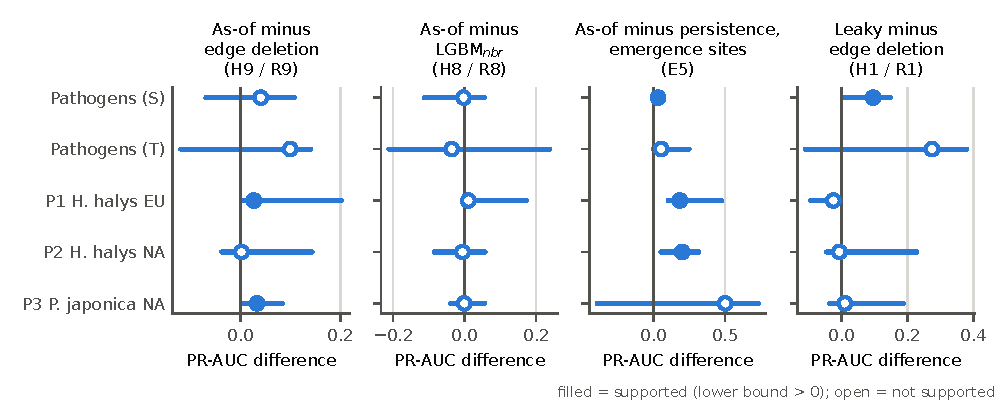
\includegraphics[width=\linewidth]{figures/fig_holdout_tests.pdf}
  \caption{Main pre-registered hold-out comparisons at the primary horizon (pathogens $N=5$, pests $N=3$): difference in PR-AUC with its 95\% block-bootstrap percentile interval. Filled markers: supported (lower bound $> 0$). Emergence sites have no target record within 50~km before the survey date.}
  \label{fig:tests}
\end{figure}

\begin{table}[t]
\centering
\caption{Hold-out PR-AUC (seed-mean score) at the primary horizon: $N=5$ for pathogens, $N=3$ for pests. Leaky models are inadmissible (they use information from the prediction window) and are shown to measure the leak. Best admissible value per column in bold.}
\label{tab:holdout}
\small
\begin{adjustbox}{max width=\linewidth}
\begin{tabular}{lccccc}
\toprule
 & \multicolumn{2}{c}{Pathogens} & \multicolumn{3}{c}{Crop pests (S)} \\
\cmidrule(lr){2-3} \cmidrule(lr){4-6}
Model & (S) & (T) & P1 \textit{H. halys} EU & P2 \textit{H. halys} NA & P3 \textit{P. japonica} NA \\
\midrule
Test sites / positives & 7{,}920 / 355 & 3{,}629 / 97 & 5{,}730 / 2{,}276 & 7{,}393 / 4{,}173 & 5{,}599 / 1{,}774 \\
Prevalence (chance)   & 0.045 & 0.027 & 0.397 & 0.564 & 0.317 \\
Persistence           & 0.258 & 0.101 & 0.836 & 0.897 & 0.570 \\
\midrule
\textbf{\Masof{} (proposed)} & 0.293 & 0.144 & 0.933 & 0.970 & 0.958 \\
\Masofplus{} (secondary)     & 0.300 & 0.180 & \textbf{0.943} & \textbf{0.976} & 0.894 \\
\Mcausal                     & 0.252 & 0.045 & 0.906 & 0.968 & 0.925 \\
\Mnoctx                      & 0.198 & 0.085 & -- & -- & -- \\
\midrule
\Lg                          & \textbf{0.363} & \textbf{0.192} & 0.891 & 0.971 & 0.947 \\
\Lnbr                        & 0.296 & 0.180 & 0.922 & \textbf{0.976} & 0.959 \\
\Lasof{} (secondary)         & 0.354 & 0.185 & 0.931 & \textbf{0.976} & \textbf{0.963} \\
\midrule
\textit{\Mleaky}             & \textit{0.348} & \textit{0.319} & \textit{0.881} & \textit{0.961} & \textit{0.935} \\
\textit{\Lleaky}             & \textit{0.387} & \textit{0.247} & \textit{0.938} & \textit{0.975} & \textit{0.964} \\
\bottomrule
\end{tabular}
\end{adjustbox}
\end{table}

\begin{table}[t]
\centering
\caption{Pre-registered hold-out differences in PR-AUC at the primary horizon, with 95\% block-bootstrap percentile intervals. $^\ast$ supported (lower bound $> 0$). Emergence: test sites without a target record within 50~km before $t_i$ (pathogens (S) 7{,}613 sites, 228 positives; (T) 3{,}575 / 79; P1 4{,}350 / 910; P2 4{,}736 / 1{,}521; P3 3{,}972 / 244).}
\label{tab:tests}
\scriptsize
\setlength{\tabcolsep}{3pt}
\begin{adjustbox}{max width=\linewidth}
\begin{tabular}{lccccc}
\toprule
Comparison & Pathogens (S) & Pathogens (T) & P1 & P2 & P3 \\
\midrule
\multicolumn{6}{l}{\textit{Proposed model (primary)}} \\
H9/R9 \Masof{} $-$ \Mcausal & $+0.040$ [$-0.069$, $0.108$] & $+0.099$ [$-0.120$, $0.140$] & $+0.026^\ast$ [$0.006$, $0.202$] & $+0.002$ [$-0.038$, $0.143$] & $+0.033^\ast$ [$0.002$, $0.084$] \\
H8/R8 \Masof{} $-$ \Lnbr & $-0.003$ [$-0.112$, $0.055$] & $-0.036$ [$-0.211$, $0.238$] & $+0.010$ [$-0.003$, $0.172$] & $-0.006$ [$-0.085$, $0.058$] & $-0.001$ [$-0.039$, $0.056$] \\
E5 \Masof{} $-$ persistence, emergence & $+0.032^\ast$ [$0.006$, $0.068$] & $+0.054$ [$-0.002$, $0.249$] & $+0.183^\ast$ [$0.103$, $0.476$] & $+0.200^\ast$ [$0.053$, $0.316$] & $+0.502$ [$-0.393$, $0.731$] \\
H7/R7 Final $-$ persistence, emergence & $+0.027^\ast$ [$0.001$, $0.074$] & $+0.008$ [$-0.006$, $0.036$] & $+0.183^\ast$ [$0.103$, $0.476$] & $+0.275^\ast$ [$0.120$, $0.301$] & $+0.428$ [$-0.017$, $0.609$] \\
H6 Final $-$ persistence, all sites & $+0.038$ [$-0.015$, $0.209$] & $+0.079$ [$-0.006$, $0.200$] & -- & -- & -- \\
\midrule
\multicolumn{6}{l}{\textit{Leakage and references (primary)}} \\
H1/R1 \Mleaky{} $-$ \Mcausal & $+0.096^\ast$ [$0.009$, $0.148$] & $+0.274$ [$-0.110$, $0.378$] & $-0.025$ [$-0.093$, $-0.010$] & $-0.007$ [$-0.046$, $0.228$] & $+0.010$ [$-0.036$, $0.187$] \\
H5/R5 \Lleaky{} $-$ \Lnbr & $+0.091$ [$-0.022$, $0.141$] & $+0.067$ [$-0.003$, $0.173$] & $+0.016$ [$-0.023$, $0.105$] & $-0.000$ [$-0.001$, $0.126$] & $+0.005$ [$-0.034$, $0.089$] \\
H2 \Mcausal{} $-$ \Lnbr & $-0.043$ [$-0.166$, $0.065$] & $-0.135$ [$-0.336$, $0.331$] & $-0.016$ [$-0.045$, $0.023$] & $-0.008$ [$-0.159$, $0.026$] & $-0.034$ [$-0.082$, $0.026$] \\
H3 \Mcausal{} $-$ \Mnoctx & $+0.054$ [$-0.165$, $0.251$] & $-0.041$ [$-0.111$, $0.337$] & -- & -- & -- \\
\midrule
\multicolumn{6}{l}{\textit{Secondary variants (designed after development results)}} \\
E1 \Masofplus{} $-$ \Mcausal & $+0.048$ [$-0.038$, $0.131$] & $+0.136$ [$-0.255$, $0.334$] & $+0.037^\ast$ [$0.017$, $0.167$] & $+0.008$ [$-0.009$, $0.184$] & $-0.031$ [$-0.312$, $0.080$] \\
E1b \Masofplus{} $-$ \Masof & $+0.008$ [$-0.027$, $0.067$] & $+0.036$ [$-0.154$, $0.207$] & $+0.010$ [$-0.053$, $0.031$] & $+0.006$ [$-0.022$, $0.056$] & $-0.064$ [$-0.326$, $0.039$] \\
E2 \Lasof{} $-$ \Lnbr & $+0.058$ [$-0.096$, $0.146$] & $+0.005$ [$-0.014$, $0.010$] & $+0.009$ [$-0.007$, $0.022$] & $-0.000$ [$-0.001$, $0.088$] & $+0.004$ [$-0.004$, $0.049$] \\
\bottomrule
\end{tabular}
\end{adjustbox}
\end{table}

\begin{itemize}[leftmargin=1.4em]

\item \textbf{Leakage Audit.}
\label{sec:audit}
Before any hold-out prediction, the diagnostics were computed on the hold-out test nodes. In the pathogen graph, 17.2\% (S) and 18.7\% (T) of the edges received by test nodes come from a later-surveyed neighbour, and 59 (S) and 22 (T) test nodes have no neighbour left in the causal graph. In the pest graphs the share is higher (32.9\%, 19.6\% and 21.9\% for P1--P3; 162, 104 and 145 isolated test nodes), and the leak is strongly associated with the label: at $N=3$, 47.2\%, 46.0\% and 56.0\% of positive test nodes receive a message containing a record from their prediction window, against 1.5\%, 1.1\% and 1.7\% of negative nodes, and this indicator alone reaches a PR-AUC of 0.660, 0.757 and 0.665 (prevalence 0.397, 0.564 and 0.317). On the development data, the gap between \Mleaky{} and \Mcausal{} was positive for every graph tested (\textit{k}-nearest-neighbour graphs with $k = 5, 10, 20$ and radius graphs of 50 and 100~km; $+0.053$ to $+0.146$ PR-AUC at $N=5$) and largest for the graphs with the most leaking edges, and among positive plots the share of later-surveyed neighbours was correlated with the gain in rank from the leaky graph (Spearman 0.374, 95\% interval $[0.204, 0.504]$). Removing a random fraction of the leaking edges did not, however, produce a monotone dose--response (slope $-0.084$, $[-0.107, 0.069]$, not supported): the loss was concentrated in removing all of them. Figure~\ref{fig:leak} summarises the audit.

\begin{figure}[pos=t]
  \centering
  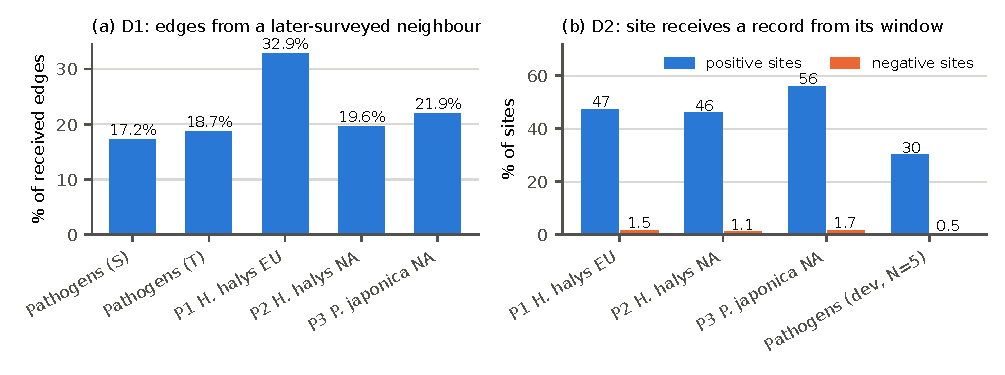
\includegraphics[width=\linewidth]{figures/fig_leak_audit.pdf}
  \caption{Leakage audit, computed from dates and records only, before any hold-out prediction. (a) D1: share of the edges received by hold-out test sites that come from a later-surveyed neighbour. (b) D2 ($N=3$, pest hold-outs): share of positive and negative test sites that receive a message containing a record from their own prediction window; pathogens: development graph at $N=5$.}
  \label{fig:leak}
\end{figure}

\item \textbf{As-of Message Passing versus Edge Deletion.}
\label{sec:mainresult}
This is the primary test of the contribution. The point estimate of \Masof{} was above the edge-deletion model in every data set (Table~\ref{tab:tests}, H9/R9). In the pest cases the difference was supported in P1 ($+0.026$, $[0.006, 0.202]$) and P3 ($+0.033$, $[0.002, 0.084]$) but not in P2 ($+0.002$), where all models are close to the ceiling (PR-AUC 0.96--0.98). The pre-registered replication criterion (supported in at least two of three cases) is therefore met. For pathogens the difference was positive in both settings ($+0.040$ in (S), $+0.099$ in (T)) but the intervals include 0, so H9 is not supported. Keeping the later neighbours with as-of features thus recovered part of the performance lost by deleting them, without any message from the prediction window.

\item \textbf{Comparison with Baselines.}
\Masof{} was neither better nor worse than the strongest admissible tabular model, \Lnbr{} (H8/R8: $-0.003$ for pathogens (S), $+0.010$, $-0.006$ and $-0.001$ for P1--P3; all intervals include 0). In contrast, the edge-deletion model was below \Lnbr{} in every data set (H2), and adding the ecological context to the causal GAT did not give a supported gain (H3). In the pathogen data set, \Lg{} without any neighbourhood feature had the highest admissible hold-out PR-AUC (0.363 in (S)), although \Lnbr{} had been better on the development data (0.456 against 0.410); the ordering of the tabular models was thus not stable between development and hold-out data.

\item \textbf{Emergence Forecasting.}
On sites without any prior record of the organism within 50~km, \Masof{} outperformed persistence for pathogens in (S) ($+0.032$, $[0.006, 0.068]$) and in pest cases P1 ($+0.183$) and P2 ($+0.200$); for P3, with 244 positive emergence sites in 20 blocks, the difference was $+0.502$ with an interval from $-0.393$ to $0.731$. The pre-registered emergence tests of the final models were supported for pathogens in (S) (H7) and replicated in pests (R7: P1 and P2). Persistence was also outperformed on all sites, although without supported differences for pathogens (H6). In setting (T), low-effort regions with 79 positive emergence sites in 27 blocks, no emergence test was supported. Figure~\ref{fig:maps} maps the hold-out risk ranks of \Masof{} next to the observed outcomes.

\begin{figure}[pos=t]
  \centering
  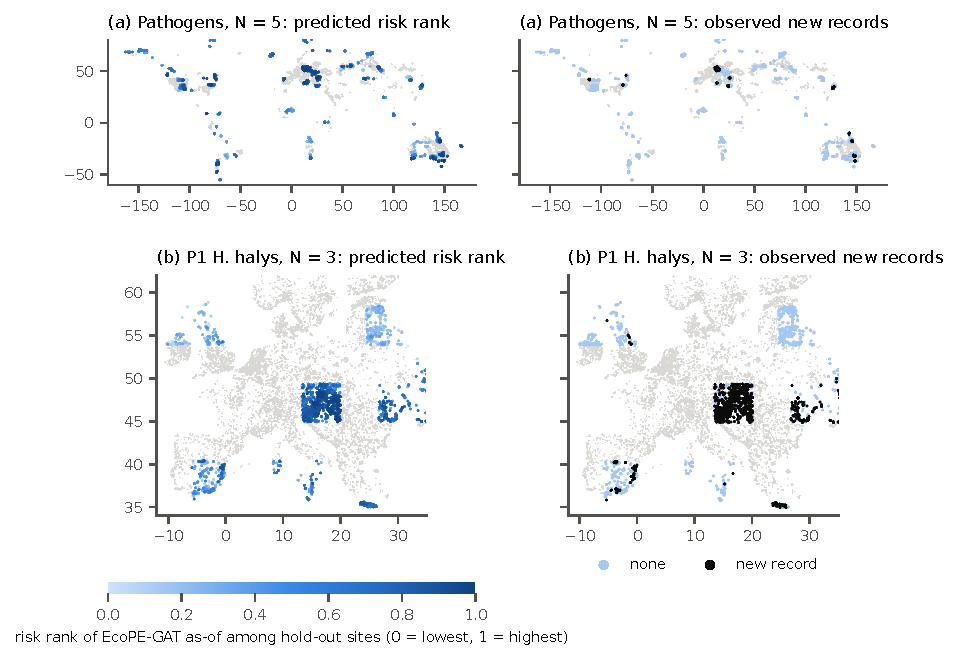
\includegraphics[width=\linewidth]{figures/fig_risk_maps.pdf}
  \caption{Hold-out forecasts of \Masof{} (seed-mean score, setting (S)). Left: rank of each hold-out site among all hold-out sites. Right: observed outcome, a new record of the target within 50~km during the prediction window. Grey: development sites. (a) Plant pathogens, $N = 5$; (b) \textit{H. halys} in Europe (P1), $N = 3$.}
  \label{fig:maps}
\end{figure}

\item \textbf{Leakage on the Hold-out.}
The leak inflated the hold-out performance of the graph model only for pathogens in setting (S): \Mleaky{} $-$ \Mcausal{} $= +0.096$, $[0.009, 0.148]$. In (T) the difference was larger but uncertain ($+0.274$, $[-0.110, 0.378]$), so the conjunction required by H1 failed. In the pest cases it was not replicated (R1), and in P1 the leaky model was significantly \emph{worse} than the causal model ($-0.025$, $[-0.093, -0.010]$), as it had already been on the development data ($-0.050$). The tabular leak (H5/R5) was not supported in any data set. The leak is therefore present in every graph (Leakage Audit), but whether a model profits from it on new data depends on the data set. Of the leakage gain observed for pathogens in (S), \Masof{} recovered 42\% (0.293 against 0.252 and 0.348), \Masofplus{} 50\% and, for the tabular models, \Lasof{} 64\% (E6, descriptive).

\item \textbf{Secondary Variants.}
Adding the 100~km and ring counts to the as-of messages did not help (E1b): \Masofplus{} was better than edge deletion only in P1 (E1), and it was unstable in P3 (0.894 against 0.958 for \Masof). Applying the as-of encoding to LightGBM neighbourhood features gave no supported gain (E2), so the general claim E3 (as-of better than removal for both graph and tabular models in at least three of four data sets) is not supported. The pre-registered choice of \Masof{} rather than \Masofplus{} as the primary model is consistent with these results.

\item \textbf{Secondary Horizons and Development Results.}
Table~\ref{tab:dev} gives the development results. On the hold-out at the secondary horizons, \Masof{} $-$ \Mcausal{} for pathogens (S) was $+0.008$ at $N=7$ and $+0.010$ at $N=10$; for pests at $N=5$ it was supported in P1 ($+0.044$, $[0.027, 0.142]$) and close to 0 in P2 and P3. At $N=5$ in P1, \Masof{} was also better than \Lnbr{} ($+0.030$, $[0.016, 0.155]$). The leaky--causal gap for pathogens (S) was $+0.119$ ($[0.031, 0.179]$) at $N=7$ and $+0.095$ ($[-0.006, 0.183]$) at $N=10$.

\begin{table}[t]
\centering
\caption{Development results: spatial cross-validation fold-mean PR-AUC of the seed-mean score (primary horizon). Descriptive; the pre-registered tests are those of Table~\ref{tab:tests}.}
\label{tab:dev}
\small
\begin{tabular}{lcccc}
\toprule
Model & Pathogens ($N=5$) & P1 ($N=3$) & P2 ($N=3$) & P3 ($N=3$) \\
\midrule
\Masof        & 0.419 & 0.868 & 0.900 & 0.942 \\
\Masofplus    & 0.416 & 0.872 & 0.903 & 0.944 \\
\Mcausal      & 0.364 & 0.811 & 0.889 & 0.929 \\
\Mnoctx       & 0.360 & -- & -- & -- \\
\Lg           & 0.410 & 0.801 & 0.895 & 0.945 \\
\Lnbr         & 0.456 & 0.855 & 0.905 & 0.948 \\
\Lasof        & 0.448 & 0.854 & 0.910 & 0.949 \\
\textit{\Mleaky} & \textit{0.478} & \textit{0.761} & \textit{0.897} & \textit{0.943} \\
\textit{\Lleaky} & \textit{0.503} & \textit{0.867} & \textit{0.920} & \textit{0.950} \\
\bottomrule
\end{tabular}
\end{table}

\item \textbf{Calibration of the Statistical Test.}
Before the hold-out run, the evaluation code was applied to random scores. With 27 test blocks in setting (T), 10 of 69 pathogen tests were ``supported'' with lower bounds between 0.000 and 0.010, and 2 of 90 pest tests; the percentile block bootstrap is therefore anti-conservative with few blocks. The frozen criterion was not changed, but results in (T) with a lower bound below 0.005 should be read as fragile. Several percentile intervals do not contain the point estimate (for example H9 in (T): $+0.099$, $[-0.120, 0.140]$), a sign of skewed bootstrap distributions when positives are concentrated in a few blocks.

\end{itemize}

% =========================================================
\section{Discussion}
\label{sec:discussion}

\subsection{As-of Message Passing as a Structural Contribution}

As-of message passing changes what a message is: instead of a property of the sending node, a message is a property of the sender evaluated at the receiver's date. The principle is the one that temporal graph networks apply to timed events \citep{xu2020tgat,rossi2020} and that point-in-time joins apply to tabular features; what is specific here is its use in static spatial graphs whose nodes store cumulative features at their own, irregular survey dates, the setting of graph SDMs. This removes the temporal leak by construction (Proposition~\ref{prop:asof}) without the cost of the standard remedy, which deletes 15--33\% of the edges in our graphs and isolates hundreds of nodes. On sealed hold-outs, the point estimate of the as-of model was above edge deletion in all four data sets, with supported and replicated differences in two of the three pest cases. The rule is simple to implement (one binary search per edge, computed once), applies to any graph model whose node features are cumulative functions of dated records, and reduces to the original features for the node itself.

\subsection{Why the GNN Approach is Justified}

The as-of model did not outperform the best tabular model: it matched \Lnbr{} in every data set, and on the pathogen hold-out a LightGBM model without neighbourhood features scored higher. A graph model is nonetheless justified for three reasons. First, under the same correction the graph model gained more than the tabular model: as-of features gave supported gains over edge deletion for the GAT in two cases, and none for LightGBM (E2). Second, \Masof{} was the final model selected by the pre-registered rule in P1 and outperformed persistence on emergence sites in three of four data sets, which is the operational question for surveillance. Third, its attention coefficients are defined on messages that are valid at the prediction date, so that the neighbours a forecast relies on can be inspected without the risk that they reflect future records.

\subsection{Transductive Bias under Spatial Holdout}

During development, we first attributed the poor geographic hold-out performance of a preliminary configuration of EcoPE-GAT to transductive training \citep{croft2023}. The present results identify a more specific bias of transductive graphs over dated sites: test nodes receive messages from neighbours whose features were computed after the test node's date. This bias is invisible to spatially blocked splits, because it passes through the model input, and it can make a graph model look better than a tabular model (on the pathogen development data, \Mleaky{} was second only to the leaky tabular model) or, as in P1, worse. Its consequences are therefore not a constant inflation but a change in what the model learns. We recommend that graph SDMs with time-stamped features report the share of edges from later neighbours (diagnostic D1, which needs only dates), the association of such edges with the labels (D2, which needs the dated source records), and the performance with and without the correction (D3).

\subsection{Ecological Interpretation}

An as-of message tells a site how many records of the organism had been reported around each of its neighbours before its own survey, that is, how close the known distribution was at the prediction date. For invasive pests spreading over a few years, this is the position of the invasion front, which explains why all models are far above chance in the pest cases and why the gains of the as-of model concentrate on emergence sites, where the site itself has no record yet (P1: +0.18 PR-AUC over persistence). For plant pathogens, prevalence is low, records are concentrated in a few well-surveyed regions and the labels record reports rather than infections; prior presence alone ranks plots far above chance, and differences between models are small relative to their uncertainty. The failure of all emergence tests in the low-effort regions (T) shows that none of the models transfers the learned spread signal to places where almost nothing is reported.

\subsection{Limitations}
\label{sec:limitations}

Despite the contributions above, several limitations should be acknowledged, which also point to directions for future work:

\begin{itemize}[leftmargin=1.4em]
  \item \textbf{Labels reflect reporting.} Labels are derived from occurrence records and confound occurrence with surveillance effort \citep{beck2014}; the independent effort layer reduces but does not remove this confounding.
  \item \textbf{Static-covariate assumption (A1).} The guarantee of Proposition~\ref{prop:asof} concerns target records. The node set and survey dates are treated as non-target covariates; in the pest cases nodes are background insect records, so the existence of a later neighbour partly reflects later sampling activity near the site.
  \item \textbf{One layer.} The as-of guarantee is exact for one attention layer; a multi-layer version would need features evaluated at the final receiver's date along every path.
  \item \textbf{Statistical power.} The hold-outs contain 19--92 blocks, and 27 blocks in the low-effort setting; the percentile block bootstrap is anti-conservative at this size, and pest PR-AUCs are close to the ceiling (P2).
  \item \textbf{Development history and pathogen hold-out.} Several preliminary configurations of EcoPE-GAT failed their pre-registered development tests (Section~\ref{sec:history}). The pathogen hold-out plots were part of exploratory pilots before they were sealed; no model, tuning or decision reported here used them. The pest hold-outs were sealed before any model was fitted.
  \item \textbf{Post hoc variants and tuning.} \Masofplus{} and \Lasof{} were designed after development results had been seen. Hyperparameters were tuned at the primary horizon and reused for the others, with reduced budgets for pests (20 trials, 3 seeds) and a subsample of 30{,}000 nodes per pest case.
  \item \textbf{Species pool.} The pathogen download covers \gbifSpecies{} well-known pathogens, many of them crop pathogens, and the pests are two species in two continents.
\end{itemize}

\subsection{Development History}
\label{sec:history}

For transparency we summarise the path that led to the present model; all steps are recorded in a decision log with version-control tags. The first configuration of EcoPE-GAT used functional-trait features on a $k$-nearest-neighbour graph in trait space, with two standard GAT layers and an MLP encoder. With an independent effort layer, traits added nothing beyond prior presence, effort and location. A pre-registered test of a second version (traits and prior presence on a combined trait and geographic graph) failed: it was not competitive with LightGBM ($-0.162$ PR-AUC, $[-0.304, +0.017]$), and the EcoPE encoder did not outperform concatenation. A pre-registered occupancy--detection extension also failed its main test. Its apparent advantage in low-effort regions was then traced to the temporal leak described here: with the causal graph, the transfer PR-AUC of the best graph model fell from 0.243 to 0.011. This finding led to the leakage hypotheses (D13), and the cost of edge deletion led to the as-of model (D14).

% =========================================================
\section{Conclusion}
\label{sec:conclusion}

We introduced as-of message passing, a rule for graph neural networks over dated sites in which each neighbour's time-stamped features are recomputed at the receiver's date, and its implementation in a graph attention network with an ecological positional encoding, \Masof. The rule keeps every edge and provably passes no record from the receiver's prediction window, whereas the standard remedy deletes up to a third of the edges. On sealed, pre-registered hold-outs, \Masof{} scored above edge deletion in all four data sets, with replicated, supported gains in two of three crop-pest cases, matched the strongest tabular model, and outperformed persistence where the organism had not yet been reported. The leak itself was present in every graph but improved hold-out performance only for pathogens in one of two settings, so reporting the correction matters more for the validity of a model than for its score. As-of message passing can be applied to any spatial graph model built from time-stamped occurrence records.

% =========================================================
\section*{Software and data availability}
\begin{itemize}[leftmargin=1.4em]
  \item \textbf{Software name:} EcoPE-GAT (code for data construction, models, pre-registered evaluation and figures).
  \item \textbf{Developers:} Mohamed Djounaid Laib and Nacéra Laiche; contact: Mohamed.djounaid.laib\_d@usthb.edu.dz.
  \item \textbf{Year first available:} 2026.
  \item \textbf{Hardware required:} standard CPU workstation; the experiments ran on a laptop with a 10-core Intel Core i5-1335U processor and 16~GB of RAM, without GPU. The single hold-out run (all refits and tests) took 6.6~h. \pending{total runtime of development tuning}
  \item \textbf{Software required:} Python 3.12 with PyTorch 2.15 (CPU), PyTorch Geometric 2.8.1, scikit-learn 1.9.1, LightGBM 4.7.0, Optuna 5.0.0, pandas 3.1.1, NumPy 2.5.5; exact versions in \texttt{requirements.txt}.
  \item \textbf{Programming language:} Python.
  \item \textbf{Program size:} \pending{lines of code}
  \item \textbf{Availability and cost:} free and open source under the MIT licence at \url{https://github.com/Laib-Djounaid/ecope}; pre-registrations, decision log and hold-out outputs are in the repository (tags \texttt{prereg-D13}, \texttt{prereg-D14}, \texttt{prereg-D15-content}, \texttt{prereg-D16}, \texttt{frozen-D16}, \texttt{holdout-results}). \pending{archived release DOI (e.g.\ Zenodo)}
\end{itemize}

\section*{Data availability}
The sPlotOpen vegetation-plot dataset is available at \url{https://doi.org/10.25829/idiv.3474-bb7k72} \citep{splotdata}. Plant-pathogen records come from the GBIF occurrence download \url{https://doi.org/10.15468/dl.ps65sp} \citep{gbifdownload}, and the independent effort layer from the GBIF SQL download \url{https://doi.org/10.15468/dl.4739rd} \citep{gbifeffort}. \pending{GBIF derived-dataset DOIs of the three crop-pest cases.} All derived data are rebuilt from these sources by the code.

\section*{Declaration of generative AI and AI-assisted technologies in the writing process}
During the preparation of this work the authors used ChatGPT (OpenAI) and Claude (Anthropic) to assist with drafting and editing the manuscript text and with writing and reviewing analysis code. After using these tools, the authors reviewed and edited the content as needed and take full responsibility for the content of the published article.

% To print the CRediT authorship contribution statement
\printcredits

\section*{Declaration of competing interest}
The authors declare that they have no known competing financial interests or personal relationships that could have appeared to influence the work reported in this paper.

\section*{Acknowledgements}
This research did not receive any specific grant from funding agencies in the public, commercial, or not-for-profit sectors.

% =========================================================
% DOIs and arXiv identifiers verified on 2026-11-16/17 (Crossref, DataCite, arXiv) and, for the
% references added in this version, on 2026-11-21 (Crossref API).
\begin{thebibliography}{99}

\bibitem{akiba2019} Akiba, T., Sano, S., Yanase, T., Ohta, T., Koyama, M. (2019). Optuna: a next-generation hyperparameter optimization framework. \textit{Proceedings of the 25th ACM SIGKDD International Conference on Knowledge Discovery \& Data Mining}, 2623--2631. DOI: \url{https://doi.org/10.1145/3292500.3330701}.

\bibitem{althoff2022} Althoff, E.R., Rice, K.B. (2022). Japanese beetle (Coleoptera: Scarabaeidae) invasion of North America: history, ecology, and management. \textit{Journal of Integrated Pest Management}, 13(1):2. DOI: \url{https://doi.org/10.1093/jipm/pmab043}.

\bibitem{bebber2014} Bebber, D.P., Holmes, T., Gurr, S.J. (2014). The global spread of crop pests and pathogens. \textit{Global Ecology and Biogeography}, 23(12):1398--1407. DOI: \url{https://doi.org/10.1111/geb.12214}.

\bibitem{beck2014} Beck, J., B\"oller, M., Erhardt, A., Schwanghart, W. (2014). Spatial bias in the GBIF database and its effect on modeling species' geographic distributions. \textit{Ecological Informatics}, 19:10--15. DOI: \url{https://doi.org/10.1016/j.ecoinf.2013.11.002}.

\bibitem{bruelheide2018} Bruelheide, H., Dengler, J., Purschke, O., et al. (2018). Global trait--environment relationships of plant communities. \textit{Nature Ecology \& Evolution}, 2(12):1906--1917. DOI: \url{https://doi.org/10.1038/s41559-018-0699-8}.

\bibitem{croft2023} Croft, V.M., van Iersel, S.C.J.L., Della Santina, C. (2023). Forecasting infections with spatio-temporal graph neural networks: a case study of the Dutch SARS-CoV-2 spread. \textit{Frontiers in Physics}, 11:1277052. DOI: \url{https://doi.org/10.3389/fphy.2023.1277052}.

\bibitem{dwivedi2020} Dwivedi, V.P., Bresson, X. (2020). A generalization of transformer networks to graphs. arXiv:2012.09699. \url{https://arxiv.org/abs/2012.09699}.

\bibitem{efron1979} Efron, B. (1979). Bootstrap methods: another look at the jackknife. \textit{The Annals of Statistics}, 7(1):1--26. DOI: \url{https://doi.org/10.1214/aos/1176344552}.

\bibitem{elith2009} Elith, J., Leathwick, J.R. (2009). Species distribution models: ecological explanation and prediction across space and time. \textit{Annual Review of Ecology, Evolution, and Systematics}, 40:677--697. DOI: \url{https://doi.org/10.1146/annurev.ecolsys.110308.120159}.

\bibitem{fey2019} Fey, M., Lenssen, J.E. (2019). Fast graph representation learning with PyTorch Geometric. arXiv:1903.02428. \url{https://arxiv.org/abs/1903.02428}.

\bibitem{fick2017} Fick, S.E., Hijmans, R.J. (2017). WorldClim 2: new 1-km spatial resolution climate surfaces for global land areas. \textit{International Journal of Climatology}, 37(12):4302--4315. DOI: \url{https://doi.org/10.1002/joc.5086}.

\bibitem{fisher2012} Fisher, M.C., Henk, D.A., Briggs, C.J., et al. (2012). Emerging fungal threats to animal, plant and ecosystem health. \textit{Nature}, 484(7393):186--194. DOI: \url{https://doi.org/10.1038/nature10947}.

\bibitem{gbifdownload} GBIF.org (2026). GBIF Occurrence Download (31 August 2026) [dataset]. DOI: \url{https://doi.org/10.15468/dl.ps65sp}.

\bibitem{gbifeffort} GBIF.org (2026). GBIF Occurrence Download, SQL query of non-target Fungi records per 0.5-degree cell and year [dataset]. DOI: \url{https://doi.org/10.15468/dl.4739rd}.

\bibitem{grinsztajn2022} Grinsztajn, L., Oyallon, E., Varoquaux, G. (2022). Why do tree-based models still outperform deep learning on typical tabular data? \textit{Advances in Neural Information Processing Systems}, 35 (Datasets and Benchmarks Track). arXiv:2207.08815.

\bibitem{guillera2015} Guillera-Arroita, G., Lahoz-Monfort, J.J., Elith, J., et al. (2015). Is my species distribution model fit for purpose? Matching data and models to applications. \textit{Global Ecology and Biogeography}, 24(3):276--292. DOI: \url{https://doi.org/10.1111/geb.12268}.

\bibitem{halliday2021} Halliday, F.W., Jalo, M., Laine, A.-L. (2021). The effect of host community functional traits on plant disease risk varies along an elevational gradient. \textit{eLife}, 10:e67340. DOI: \url{https://doi.org/10.7554/eLife.67340}.

\bibitem{hamilton2017} Hamilton, W.L., Ying, R., Leskovec, J. (2017). Inductive representation learning on large graphs. \textit{Advances in Neural Information Processing Systems}, 30. arXiv:1706.02216.

\bibitem{harrell2025} Harrell, L., Kaeser-Chen, C., Karagol Ayan, B., et al. (2025). Heterogeneous graph neural networks for species distribution modeling. \textit{ICLR 2025 Workshop on Tackling Climate Change with Machine Learning}. arXiv:2503.11900.

\bibitem{hijmans2012} Hijmans, R.J. (2012). Cross-validation of species distribution models: removing spatial sorting bias and calibration with a null model. \textit{Ecology}, 93(3):679--688. DOI: \url{https://doi.org/10.1890/11-0826.1}.

\bibitem{huang2023} Huang, S., Poursafaei, F., Danovitch, J., et al. (2023). Temporal graph benchmark for machine learning on temporal graphs. \textit{Advances in Neural Information Processing Systems}, 36 (Datasets and Benchmarks Track). arXiv:2307.01026.

\bibitem{jin2021} Jin, H., Yuan, Y., Li, J. (2021). Host functional traits affect plant responses to pathogen stress: a meta-analysis. \textit{Acta Oecologica}, 110:103703. DOI: \url{https://doi.org/10.1016/j.actao.2021.103703}.

\bibitem{kapoor2023} Kapoor, S., Narayanan, A. (2023). Leakage and the reproducibility crisis in machine-learning-based science. \textit{Patterns}, 4(9):100804. DOI: \url{https://doi.org/10.1016/j.patter.2023.100804}.

\bibitem{kaufman2012} Kaufman, S., Rosset, S., Perlich, C., Stitelman, O. (2012). Leakage in data mining: formulation, detection, and avoidance. \textit{ACM Transactions on Knowledge Discovery from Data}, 6(4):1--21. DOI: \url{https://doi.org/10.1145/2382577.2382579}.

\bibitem{ke2017} Ke, G., Meng, Q., Finley, T., Wang, T., Chen, W., Ma, W., Ye, Q., Liu, T.-Y. (2017). LightGBM: a highly efficient gradient boosting decision tree. \textit{Advances in Neural Information Processing Systems}, 30:3146--3154.

\bibitem{kingma2015} Kingma, D.P., Ba, J. (2015). Adam: a method for stochastic optimization. \textit{International Conference on Learning Representations (ICLR)}. arXiv:1412.6980.

\bibitem{kipf2017} Kipf, T.N., Welling, M. (2017). Semi-supervised classification with graph convolutional networks. \textit{International Conference on Learning Representations (ICLR)}. arXiv:1609.02907.

\bibitem{klemmer2023pegnn} Klemmer, K., Safir, N.S., Neill, D.B. (2023). Positional encoder graph neural networks for geographic data. \textit{Proceedings of the 26th International Conference on Artificial Intelligence and Statistics (AISTATS)}, PMLR 206:1379--1389.

\bibitem{kong2026} Kong, S., Yu, T., Wei, Y., Liu, C., Bai, J., Wang, Y., Grimson, M., Fink, D. (2026). STELLAR: spatio-temporal environmental learning with latent alignment and refinement for long-tailed species distribution modeling. arXiv:2606.08484. \url{https://arxiv.org/abs/2606.08484}.

\bibitem{kumar2019} Kumar, S., Zhang, X., Leskovec, J. (2019). Predicting dynamic embedding trajectory in temporal interaction networks. \textit{Proceedings of the 25th ACM SIGKDD International Conference on Knowledge Discovery \& Data Mining}, 1269--1278. DOI: \url{https://doi.org/10.1145/3292500.3330895}.

\bibitem{lavorel2002} Lavorel, S., Garnier, E. (2002). Predicting changes in community composition and ecosystem functioning from plant traits: revisiting the Holy Grail. \textit{Functional Ecology}, 16(5):545--556. DOI: \url{https://doi.org/10.1046/j.1365-2435.2002.00664.x}.

\bibitem{leskey2018} Leskey, T.C., Nielsen, A.L. (2018). Impact of the invasive brown marmorated stink bug in North America and Europe: history, biology, ecology, and management. \textit{Annual Review of Entomology}, 63:599--618. DOI: \url{https://doi.org/10.1146/annurev-ento-020117-043226}.

\bibitem{li2020} Li, P., Wang, Y., Wang, H., Leskovec, J. (2020). Distance encoding: design provably more powerful neural networks for graph representation learning. \textit{Advances in Neural Information Processing Systems}, 33. arXiv:2009.00142.

\bibitem{maganti2026} Maganti, S. (2026). When graph structure becomes a liability: a critical re-evaluation of graph neural networks for Bitcoin fraud detection under temporal distribution shift. arXiv:2604.19514. \url{https://arxiv.org/abs/2604.19514}.

\bibitem{meyer2018} Meyer, H., Reudenbach, C., Hengl, T., Katurji, M., Nauss, T. (2018). Improving performance of spatio-temporal machine learning models using forward feature selection and target-oriented validation. \textit{Environmental Modelling \& Software}, 101:1--9. DOI: \url{https://doi.org/10.1016/j.envsoft.2017.12.001}.

\bibitem{nosek2018} Nosek, B.A., Ebersole, C.R., DeHaven, A.C., Mellor, D.T. (2018). The preregistration revolution. \textit{Proceedings of the National Academy of Sciences}, 115(11):2600--2606. DOI: \url{https://doi.org/10.1073/pnas.1708274114}.

\bibitem{paszke2019} Paszke, A., Gross, S., Massa, F., et al. (2019). PyTorch: an imperative style, high-performance deep learning library. \textit{Advances in Neural Information Processing Systems}, 32. arXiv:1912.01703.

\bibitem{pedregosa2011} Pedregosa, F., Varoquaux, G., Gramfort, A., et al. (2011). Scikit-learn: machine learning in Python. \textit{Journal of Machine Learning Research}, 12:2825--2830.

\bibitem{phillips2009} Phillips, S.J., Dud\'ik, M., Elith, J., Graham, C.H., Lehmann, A., Leathwick, J., Ferrier, S. (2009). Sample selection bias and presence-only distribution models: implications for background and pseudo-absence data. \textit{Ecological Applications}, 19(1):181--197. DOI: \url{https://doi.org/10.1890/07-2153.1}.

\bibitem{ploton2020} Ploton, P., Mortier, F., R\'ejou-M\'echain, M., et al. (2020). Spatial validation reveals poor predictive performance of large-scale ecological mapping models. \textit{Nature Communications}, 11:4540. DOI: \url{https://doi.org/10.1038/s41467-020-18321-y}.

\bibitem{poursafaei2022} Poursafaei, F., Huang, S., Pelrine, K., Rabbany, R. (2022). Towards better evaluation for dynamic link prediction. \textit{Advances in Neural Information Processing Systems}, 35 (Datasets and Benchmarks Track). arXiv:2207.10128.

\bibitem{roberts2017} Roberts, D.R., Bahn, V., Ciuti, S., et al. (2017). Cross-validation strategies for data with temporal, spatial, hierarchical, or phylogenetic structure. \textit{Ecography}, 40(8):913--929. DOI: \url{https://doi.org/10.1111/ecog.02881}.

\bibitem{rossi2020} Rossi, E., Chamberlain, B., Frasca, F., Eynard, D., Monti, F., Bronstein, M. (2020). Temporal graph networks for deep learning on dynamic graphs. arXiv:2006.10637. \url{https://arxiv.org/abs/2006.10637}.

\bibitem{sabatini2021} Sabatini, F.M., Lenoir, J., Hattab, T., et al. (2021). sPlotOpen -- an environmentally balanced, open-access, global dataset of vegetation plots. \textit{Global Ecology and Biogeography}, 30(9):1740--1764. DOI: \url{https://doi.org/10.1111/geb.13346}.

\bibitem{splotdata} Sabatini, F.M., Lenoir, J., Bruelheide, H. (2021). sPlotOpen -- an environmentally-balanced, open-access, global dataset of vegetation plots [dataset]. German Centre for Integrative Biodiversity Research (iDiv) Halle-Jena-Leipzig. DOI: \url{https://doi.org/10.25829/idiv.3474-bb7k72}.

\bibitem{saito2015} Saito, T., Rehmsmeier, M. (2015). The precision-recall plot is more informative than the ROC plot when evaluating binary classifiers on imbalanced datasets. \textit{PLOS ONE}, 10(3):e0118432. DOI: \url{https://doi.org/10.1371/journal.pone.0118432}.

\bibitem{siefert2024} Siefert, A., Laughlin, D.C., Sabatini, F.M. (2024). You shall know a species by the company it keeps: leveraging co-occurrence data to improve ecological prediction. \textit{Journal of Vegetation Science}, 35:e13314. DOI: \url{https://doi.org/10.1111/jvs.13314}.

\bibitem{valavi2019} Valavi, R., Elith, J., Lahoz-Monfort, J.J., Guillera-Arroita, G. (2019). blockCV: an R package for generating spatially or environmentally separated folds for k-fold cross-validation of species distribution models. \textit{Methods in Ecology and Evolution}, 10(2):225--232. DOI: \url{https://doi.org/10.1111/2041-210X.13107}.

\bibitem{valavi2022} Valavi, R., Guillera-Arroita, G., Lahoz-Monfort, J.J., Elith, J. (2022). Predictive performance of presence-only species distribution models: a benchmark study with reproducible code. \textit{Ecological Monographs}, 92(1):e01486. DOI: \url{https://doi.org/10.1002/ecm.1486}.

\bibitem{velickovic2018} Veli\v{c}kovi\'c, P., Cucurull, G., Casanova, A., Romero, A., Li\`o, P., Bengio, Y. (2018). Graph attention networks. \textit{International Conference on Learning Representations (ICLR)}. arXiv:1710.10903.

\bibitem{wadoux2021} Wadoux, A.M.J.-C., Heuvelink, G.B.M., de Bruin, S., Brus, D.J. (2021). Spatial cross-validation is not the right way to evaluate map accuracy. \textit{Ecological Modelling}, 457:109692. DOI: \url{https://doi.org/10.1016/j.ecolmodel.2021.109692}.

\bibitem{wu2025} Wu, Z., Wang, J., Wu, H., Li, S., Dai, W. (2025). GNN-SDM: a graph neural network-based framework integrating complex landscape patterns into species distribution modelling. \textit{Global Ecology and Biogeography}, 34:e70162. DOI: \url{https://doi.org/10.1111/geb.70162}.

\bibitem{xu2020tgat} Xu, D., Ruan, C., Korpeoglu, E., Kumar, S., Achan, K. (2020). Inductive representation learning on temporal graphs. \textit{International Conference on Learning Representations (ICLR)}. arXiv:2002.07962.

\bibitem{yates2018} Yates, K.L., Bouchet, P.J., Caley, M.J., et al. (2018). Outstanding challenges in the transferability of ecological models. \textit{Trends in Ecology \& Evolution}, 33(10):790--802. DOI: \url{https://doi.org/10.1016/j.tree.2018.08.001}.

\bibitem{zhou2026} Zhou, H., Li, Y., Yang, J., Hu, H., Wang, C., Liu, H., Lin, Y. (2026). Multi-graph spatial--temporal graph convolutional networks for predicting the spread of \textit{Dendroctonus valens} in China. \textit{Journal of Forestry Research}, 37:153. DOI: \url{https://doi.org/10.1007/s11676-026-02097-w}.

\bibitem{zhao2023} Zhao, W., Efremova, N. (2023). Soil organic carbon estimation from climate-related features with graph neural network. arXiv:2311.15979.

\end{thebibliography}
\end{document}
